\documentclass[11pt]{article}

% Shared notes settings for Applied Machine Learning lectures (UPES).
% Keep this file free of \documentclass to allow reuse via \input.

\usepackage[utf8]{inputenc}
\usepackage[T1]{fontenc}
\usepackage{lmodern}          % scalable T1 fonts; without this pdflatex falls back
\input{glyphtounicode}        % to bitmapped EC Type 3 and the PDFs are neither
\pdfgentounicode=1            % searchable nor screen-reader friendly
\usepackage[a4paper,margin=1in]{geometry}
\usepackage{hyperref}
\usepackage{xurl}
\usepackage{booktabs}
\usepackage{amsmath}
\usepackage{amssymb}
\usepackage{listings}
\usepackage{xcolor}
\usepackage{enumitem}
\usepackage{parskip}

% Code listings (Python-oriented for this subject).
\lstset{
  language=Python,
  basicstyle=\ttfamily\small,
  keywordstyle=\color{blue},
  commentstyle=\color{gray},
  stringstyle=\color{teal},
  showstringspaces=false,
  columns=fullflexible,
  frame=single,
  framerule=0.2pt,
  breaklines=true
}

\setlist[itemize]{topsep=0.3em,itemsep=0.2em}
\setlist[enumerate]{topsep=0.3em,itemsep=0.2em}

% Simple per-section source line.
\newcommand{\notesources}[1]{\par\noindent{\small\color{gray}\textit{Sources:} \sloppy #1\par}}

% Unit-wise source strings for this subject (used by slides + notes).
% Path is relative to the lecture `latex/` folder (the compilation CWD).
\IfFileExists{../../../_shared/aml-sources.tex}{%
  % Source strings for Applied Machine Learning (CSAI2017P) — used by slides + notes.
% Prescribed texts and reference books are taken from the course syllabus.
% Support texts are the author-hosted open-access editions:
%   statlearning.com            (ISL with Python)
%   probml.github.io/pml-book   (Murphy, Probabilistic Machine Learning)
%   d2l.ai                      (Dive into Deep Learning)
%   mml-book.github.io          (Mathematics for Machine Learning)

\newcommand{\AMLRepoURL}{https://github.com/tali7c/Applied-Machine-Learning}

% --- prescribed -------------------------------------------------------------
\newcommand{\AMLPrescribed}{%
M\"uller and Guido, \textit{Introduction to Machine Learning with Python}, O'Reilly, 2016.;%
Bishop, \textit{Pattern Recognition and Machine Learning}, Springer, 2006.;%
Murphy, \textit{Machine Learning: A Probabilistic Perspective}, MIT Press, 2012.;%
Han, Kamber and Pei, \textit{Data Mining: Concepts and Techniques} (3e), Morgan Kaufmann, 2012.%
}

% --- unit-wise ---------------------------------------------------------------
\newcommand{\AMLUnitISources}{%
M\"uller and Guido, \textit{Introduction to Machine Learning with Python}, Ch. 1.;%
Bishop, \textit{Pattern Recognition and Machine Learning}, Ch. 1.;%
Murphy, \textit{Probabilistic Machine Learning: An Introduction}, MIT Press, 2022, Ch. 1.;%
Mitchell, \textit{Machine Learning}, McGraw Hill, 1997, Ch. 1.;%
Scikit-learn documentation, accessed 2026-08-04.%
}

\newcommand{\AMLUnitIISources}{%
Bishop, \textit{Pattern Recognition and Machine Learning}, \S1.5, \S4.3, \S7.1.;%
Zhang, Lipton, Li and Smola, \textit{Dive into Deep Learning}, \S3.4.;%
Shalev-Shwartz and Ben-David, \textit{Understanding Machine Learning}, Ch. 15.;%
Murphy, \textit{Probabilistic Machine Learning: An Introduction}, Ch. 5.%
}

\newcommand{\AMLUnitIIISources}{%
Zhang, Lipton, Li and Smola, \textit{Dive into Deep Learning}, Ch. 12 (Optimization Algorithms).;%
Deisenroth, Faisal and Ong, \textit{Mathematics for Machine Learning}, Ch. 7.;%
Kingma and Ba, ``Adam: A Method for Stochastic Optimization,'' ICLR 2015.;%
Ruder, ``An overview of gradient descent optimization algorithms,'' arXiv:1609.04747, 2016.%
}

\newcommand{\AMLUnitIVSources}{%
Han, Kamber and Pei, \textit{Data Mining: Concepts and Techniques} (3e), Ch. 3.;%
M\"uller and Guido, \textit{Introduction to Machine Learning with Python}, Ch. 3--4.;%
James, Witten, Hastie, Tibshirani and Taylor, \textit{An Introduction to Statistical Learning with Python}, Ch. 5--6, 12.;%
Scikit-learn documentation (preprocessing, model selection), accessed 2026-08-04.%
}

\newcommand{\AMLUnitVSources}{%
James et al., \textit{An Introduction to Statistical Learning with Python}, Ch. 3--6.;%
Bishop, \textit{Pattern Recognition and Machine Learning}, Ch. 3.;%
Deisenroth, Faisal and Ong, \textit{Mathematics for Machine Learning}, Ch. 9.;%
M\"uller and Guido, \textit{Introduction to Machine Learning with Python}, \S2.3.%
}

\newcommand{\AMLUnitVISources}{%
Han, Kamber and Pei, \textit{Data Mining: Concepts and Techniques} (3e), Ch. 8--9.;%
James et al., \textit{An Introduction to Statistical Learning with Python}, Ch. 8--9.;%
Bishop, \textit{Pattern Recognition and Machine Learning}, Ch. 4--5, 7, 14.;%
Zhang et al., \textit{Dive into Deep Learning}, Ch. 5.%
}

\newcommand{\AMLUnitVIISources}{%
Han, Kamber and Pei, \textit{Data Mining: Concepts and Techniques} (3e), Ch. 10.;%
James et al., \textit{An Introduction to Statistical Learning with Python}, Ch. 12.;%
M\"uller and Guido, \textit{Introduction to Machine Learning with Python}, \S3.5.;%
Ester, Kriegel, Sander and Xu, ``A density-based algorithm for discovering clusters (DBSCAN),'' KDD 1996.%
}

\newcommand{\AMLLabSources}{%
M\"uller and Guido, \textit{Introduction to Machine Learning with Python}, companion notebooks.;%
McKinney, \textit{Python for Data Analysis} (3e), O'Reilly, 2022.;%
Scikit-learn user guide, accessed 2026-08-04.;%
Matplotlib and Seaborn documentation, accessed 2026-08-04.%
}
%
}{%
  % Faculty copies live under `private/` so their compile CWD is different.
  \IfFileExists{../../../../public/_shared/aml-sources.tex}{%
    % Source strings for Applied Machine Learning (CSAI2017P) — used by slides + notes.
% Prescribed texts and reference books are taken from the course syllabus.
% Support texts are the author-hosted open-access editions:
%   statlearning.com            (ISL with Python)
%   probml.github.io/pml-book   (Murphy, Probabilistic Machine Learning)
%   d2l.ai                      (Dive into Deep Learning)
%   mml-book.github.io          (Mathematics for Machine Learning)

\newcommand{\AMLRepoURL}{https://github.com/tali7c/Applied-Machine-Learning}

% --- prescribed -------------------------------------------------------------
\newcommand{\AMLPrescribed}{%
M\"uller and Guido, \textit{Introduction to Machine Learning with Python}, O'Reilly, 2016.;%
Bishop, \textit{Pattern Recognition and Machine Learning}, Springer, 2006.;%
Murphy, \textit{Machine Learning: A Probabilistic Perspective}, MIT Press, 2012.;%
Han, Kamber and Pei, \textit{Data Mining: Concepts and Techniques} (3e), Morgan Kaufmann, 2012.%
}

% --- unit-wise ---------------------------------------------------------------
\newcommand{\AMLUnitISources}{%
M\"uller and Guido, \textit{Introduction to Machine Learning with Python}, Ch. 1.;%
Bishop, \textit{Pattern Recognition and Machine Learning}, Ch. 1.;%
Murphy, \textit{Probabilistic Machine Learning: An Introduction}, MIT Press, 2022, Ch. 1.;%
Mitchell, \textit{Machine Learning}, McGraw Hill, 1997, Ch. 1.;%
Scikit-learn documentation, accessed 2026-08-04.%
}

\newcommand{\AMLUnitIISources}{%
Bishop, \textit{Pattern Recognition and Machine Learning}, \S1.5, \S4.3, \S7.1.;%
Zhang, Lipton, Li and Smola, \textit{Dive into Deep Learning}, \S3.4.;%
Shalev-Shwartz and Ben-David, \textit{Understanding Machine Learning}, Ch. 15.;%
Murphy, \textit{Probabilistic Machine Learning: An Introduction}, Ch. 5.%
}

\newcommand{\AMLUnitIIISources}{%
Zhang, Lipton, Li and Smola, \textit{Dive into Deep Learning}, Ch. 12 (Optimization Algorithms).;%
Deisenroth, Faisal and Ong, \textit{Mathematics for Machine Learning}, Ch. 7.;%
Kingma and Ba, ``Adam: A Method for Stochastic Optimization,'' ICLR 2015.;%
Ruder, ``An overview of gradient descent optimization algorithms,'' arXiv:1609.04747, 2016.%
}

\newcommand{\AMLUnitIVSources}{%
Han, Kamber and Pei, \textit{Data Mining: Concepts and Techniques} (3e), Ch. 3.;%
M\"uller and Guido, \textit{Introduction to Machine Learning with Python}, Ch. 3--4.;%
James, Witten, Hastie, Tibshirani and Taylor, \textit{An Introduction to Statistical Learning with Python}, Ch. 5--6, 12.;%
Scikit-learn documentation (preprocessing, model selection), accessed 2026-08-04.%
}

\newcommand{\AMLUnitVSources}{%
James et al., \textit{An Introduction to Statistical Learning with Python}, Ch. 3--6.;%
Bishop, \textit{Pattern Recognition and Machine Learning}, Ch. 3.;%
Deisenroth, Faisal and Ong, \textit{Mathematics for Machine Learning}, Ch. 9.;%
M\"uller and Guido, \textit{Introduction to Machine Learning with Python}, \S2.3.%
}

\newcommand{\AMLUnitVISources}{%
Han, Kamber and Pei, \textit{Data Mining: Concepts and Techniques} (3e), Ch. 8--9.;%
James et al., \textit{An Introduction to Statistical Learning with Python}, Ch. 8--9.;%
Bishop, \textit{Pattern Recognition and Machine Learning}, Ch. 4--5, 7, 14.;%
Zhang et al., \textit{Dive into Deep Learning}, Ch. 5.%
}

\newcommand{\AMLUnitVIISources}{%
Han, Kamber and Pei, \textit{Data Mining: Concepts and Techniques} (3e), Ch. 10.;%
James et al., \textit{An Introduction to Statistical Learning with Python}, Ch. 12.;%
M\"uller and Guido, \textit{Introduction to Machine Learning with Python}, \S3.5.;%
Ester, Kriegel, Sander and Xu, ``A density-based algorithm for discovering clusters (DBSCAN),'' KDD 1996.%
}

\newcommand{\AMLLabSources}{%
M\"uller and Guido, \textit{Introduction to Machine Learning with Python}, companion notebooks.;%
McKinney, \textit{Python for Data Analysis} (3e), O'Reilly, 2022.;%
Scikit-learn user guide, accessed 2026-08-04.;%
Matplotlib and Seaborn documentation, accessed 2026-08-04.%
}
%
  }{%
    % Question papers live at `private/<family>/<instrument>/`.
    \IfFileExists{../../../public/_shared/aml-sources.tex}{%
      % Source strings for Applied Machine Learning (CSAI2017P) — used by slides + notes.
% Prescribed texts and reference books are taken from the course syllabus.
% Support texts are the author-hosted open-access editions:
%   statlearning.com            (ISL with Python)
%   probml.github.io/pml-book   (Murphy, Probabilistic Machine Learning)
%   d2l.ai                      (Dive into Deep Learning)
%   mml-book.github.io          (Mathematics for Machine Learning)

\newcommand{\AMLRepoURL}{https://github.com/tali7c/Applied-Machine-Learning}

% --- prescribed -------------------------------------------------------------
\newcommand{\AMLPrescribed}{%
M\"uller and Guido, \textit{Introduction to Machine Learning with Python}, O'Reilly, 2016.;%
Bishop, \textit{Pattern Recognition and Machine Learning}, Springer, 2006.;%
Murphy, \textit{Machine Learning: A Probabilistic Perspective}, MIT Press, 2012.;%
Han, Kamber and Pei, \textit{Data Mining: Concepts and Techniques} (3e), Morgan Kaufmann, 2012.%
}

% --- unit-wise ---------------------------------------------------------------
\newcommand{\AMLUnitISources}{%
M\"uller and Guido, \textit{Introduction to Machine Learning with Python}, Ch. 1.;%
Bishop, \textit{Pattern Recognition and Machine Learning}, Ch. 1.;%
Murphy, \textit{Probabilistic Machine Learning: An Introduction}, MIT Press, 2022, Ch. 1.;%
Mitchell, \textit{Machine Learning}, McGraw Hill, 1997, Ch. 1.;%
Scikit-learn documentation, accessed 2026-08-04.%
}

\newcommand{\AMLUnitIISources}{%
Bishop, \textit{Pattern Recognition and Machine Learning}, \S1.5, \S4.3, \S7.1.;%
Zhang, Lipton, Li and Smola, \textit{Dive into Deep Learning}, \S3.4.;%
Shalev-Shwartz and Ben-David, \textit{Understanding Machine Learning}, Ch. 15.;%
Murphy, \textit{Probabilistic Machine Learning: An Introduction}, Ch. 5.%
}

\newcommand{\AMLUnitIIISources}{%
Zhang, Lipton, Li and Smola, \textit{Dive into Deep Learning}, Ch. 12 (Optimization Algorithms).;%
Deisenroth, Faisal and Ong, \textit{Mathematics for Machine Learning}, Ch. 7.;%
Kingma and Ba, ``Adam: A Method for Stochastic Optimization,'' ICLR 2015.;%
Ruder, ``An overview of gradient descent optimization algorithms,'' arXiv:1609.04747, 2016.%
}

\newcommand{\AMLUnitIVSources}{%
Han, Kamber and Pei, \textit{Data Mining: Concepts and Techniques} (3e), Ch. 3.;%
M\"uller and Guido, \textit{Introduction to Machine Learning with Python}, Ch. 3--4.;%
James, Witten, Hastie, Tibshirani and Taylor, \textit{An Introduction to Statistical Learning with Python}, Ch. 5--6, 12.;%
Scikit-learn documentation (preprocessing, model selection), accessed 2026-08-04.%
}

\newcommand{\AMLUnitVSources}{%
James et al., \textit{An Introduction to Statistical Learning with Python}, Ch. 3--6.;%
Bishop, \textit{Pattern Recognition and Machine Learning}, Ch. 3.;%
Deisenroth, Faisal and Ong, \textit{Mathematics for Machine Learning}, Ch. 9.;%
M\"uller and Guido, \textit{Introduction to Machine Learning with Python}, \S2.3.%
}

\newcommand{\AMLUnitVISources}{%
Han, Kamber and Pei, \textit{Data Mining: Concepts and Techniques} (3e), Ch. 8--9.;%
James et al., \textit{An Introduction to Statistical Learning with Python}, Ch. 8--9.;%
Bishop, \textit{Pattern Recognition and Machine Learning}, Ch. 4--5, 7, 14.;%
Zhang et al., \textit{Dive into Deep Learning}, Ch. 5.%
}

\newcommand{\AMLUnitVIISources}{%
Han, Kamber and Pei, \textit{Data Mining: Concepts and Techniques} (3e), Ch. 10.;%
James et al., \textit{An Introduction to Statistical Learning with Python}, Ch. 12.;%
M\"uller and Guido, \textit{Introduction to Machine Learning with Python}, \S3.5.;%
Ester, Kriegel, Sander and Xu, ``A density-based algorithm for discovering clusters (DBSCAN),'' KDD 1996.%
}

\newcommand{\AMLLabSources}{%
M\"uller and Guido, \textit{Introduction to Machine Learning with Python}, companion notebooks.;%
McKinney, \textit{Python for Data Analysis} (3e), O'Reilly, 2022.;%
Scikit-learn user guide, accessed 2026-08-04.;%
Matplotlib and Seaborn documentation, accessed 2026-08-04.%
}
%
    }{%
      % Marking schemes live at `private/solutions/<family>/<id>/latex/`.
      \IfFileExists{../../../../../public/_shared/aml-sources.tex}{%
        % Source strings for Applied Machine Learning (CSAI2017P) — used by slides + notes.
% Prescribed texts and reference books are taken from the course syllabus.
% Support texts are the author-hosted open-access editions:
%   statlearning.com            (ISL with Python)
%   probml.github.io/pml-book   (Murphy, Probabilistic Machine Learning)
%   d2l.ai                      (Dive into Deep Learning)
%   mml-book.github.io          (Mathematics for Machine Learning)

\newcommand{\AMLRepoURL}{https://github.com/tali7c/Applied-Machine-Learning}

% --- prescribed -------------------------------------------------------------
\newcommand{\AMLPrescribed}{%
M\"uller and Guido, \textit{Introduction to Machine Learning with Python}, O'Reilly, 2016.;%
Bishop, \textit{Pattern Recognition and Machine Learning}, Springer, 2006.;%
Murphy, \textit{Machine Learning: A Probabilistic Perspective}, MIT Press, 2012.;%
Han, Kamber and Pei, \textit{Data Mining: Concepts and Techniques} (3e), Morgan Kaufmann, 2012.%
}

% --- unit-wise ---------------------------------------------------------------
\newcommand{\AMLUnitISources}{%
M\"uller and Guido, \textit{Introduction to Machine Learning with Python}, Ch. 1.;%
Bishop, \textit{Pattern Recognition and Machine Learning}, Ch. 1.;%
Murphy, \textit{Probabilistic Machine Learning: An Introduction}, MIT Press, 2022, Ch. 1.;%
Mitchell, \textit{Machine Learning}, McGraw Hill, 1997, Ch. 1.;%
Scikit-learn documentation, accessed 2026-08-04.%
}

\newcommand{\AMLUnitIISources}{%
Bishop, \textit{Pattern Recognition and Machine Learning}, \S1.5, \S4.3, \S7.1.;%
Zhang, Lipton, Li and Smola, \textit{Dive into Deep Learning}, \S3.4.;%
Shalev-Shwartz and Ben-David, \textit{Understanding Machine Learning}, Ch. 15.;%
Murphy, \textit{Probabilistic Machine Learning: An Introduction}, Ch. 5.%
}

\newcommand{\AMLUnitIIISources}{%
Zhang, Lipton, Li and Smola, \textit{Dive into Deep Learning}, Ch. 12 (Optimization Algorithms).;%
Deisenroth, Faisal and Ong, \textit{Mathematics for Machine Learning}, Ch. 7.;%
Kingma and Ba, ``Adam: A Method for Stochastic Optimization,'' ICLR 2015.;%
Ruder, ``An overview of gradient descent optimization algorithms,'' arXiv:1609.04747, 2016.%
}

\newcommand{\AMLUnitIVSources}{%
Han, Kamber and Pei, \textit{Data Mining: Concepts and Techniques} (3e), Ch. 3.;%
M\"uller and Guido, \textit{Introduction to Machine Learning with Python}, Ch. 3--4.;%
James, Witten, Hastie, Tibshirani and Taylor, \textit{An Introduction to Statistical Learning with Python}, Ch. 5--6, 12.;%
Scikit-learn documentation (preprocessing, model selection), accessed 2026-08-04.%
}

\newcommand{\AMLUnitVSources}{%
James et al., \textit{An Introduction to Statistical Learning with Python}, Ch. 3--6.;%
Bishop, \textit{Pattern Recognition and Machine Learning}, Ch. 3.;%
Deisenroth, Faisal and Ong, \textit{Mathematics for Machine Learning}, Ch. 9.;%
M\"uller and Guido, \textit{Introduction to Machine Learning with Python}, \S2.3.%
}

\newcommand{\AMLUnitVISources}{%
Han, Kamber and Pei, \textit{Data Mining: Concepts and Techniques} (3e), Ch. 8--9.;%
James et al., \textit{An Introduction to Statistical Learning with Python}, Ch. 8--9.;%
Bishop, \textit{Pattern Recognition and Machine Learning}, Ch. 4--5, 7, 14.;%
Zhang et al., \textit{Dive into Deep Learning}, Ch. 5.%
}

\newcommand{\AMLUnitVIISources}{%
Han, Kamber and Pei, \textit{Data Mining: Concepts and Techniques} (3e), Ch. 10.;%
James et al., \textit{An Introduction to Statistical Learning with Python}, Ch. 12.;%
M\"uller and Guido, \textit{Introduction to Machine Learning with Python}, \S3.5.;%
Ester, Kriegel, Sander and Xu, ``A density-based algorithm for discovering clusters (DBSCAN),'' KDD 1996.%
}

\newcommand{\AMLLabSources}{%
M\"uller and Guido, \textit{Introduction to Machine Learning with Python}, companion notebooks.;%
McKinney, \textit{Python for Data Analysis} (3e), O'Reilly, 2022.;%
Scikit-learn user guide, accessed 2026-08-04.;%
Matplotlib and Seaborn documentation, accessed 2026-08-04.%
}
%
      }{%
        % Source strings for Applied Machine Learning (CSAI2017P) — used by slides + notes.
% Prescribed texts and reference books are taken from the course syllabus.
% Support texts are the author-hosted open-access editions:
%   statlearning.com            (ISL with Python)
%   probml.github.io/pml-book   (Murphy, Probabilistic Machine Learning)
%   d2l.ai                      (Dive into Deep Learning)
%   mml-book.github.io          (Mathematics for Machine Learning)

\newcommand{\AMLRepoURL}{https://github.com/tali7c/Applied-Machine-Learning}

% --- prescribed -------------------------------------------------------------
\newcommand{\AMLPrescribed}{%
M\"uller and Guido, \textit{Introduction to Machine Learning with Python}, O'Reilly, 2016.;%
Bishop, \textit{Pattern Recognition and Machine Learning}, Springer, 2006.;%
Murphy, \textit{Machine Learning: A Probabilistic Perspective}, MIT Press, 2012.;%
Han, Kamber and Pei, \textit{Data Mining: Concepts and Techniques} (3e), Morgan Kaufmann, 2012.%
}

% --- unit-wise ---------------------------------------------------------------
\newcommand{\AMLUnitISources}{%
M\"uller and Guido, \textit{Introduction to Machine Learning with Python}, Ch. 1.;%
Bishop, \textit{Pattern Recognition and Machine Learning}, Ch. 1.;%
Murphy, \textit{Probabilistic Machine Learning: An Introduction}, MIT Press, 2022, Ch. 1.;%
Mitchell, \textit{Machine Learning}, McGraw Hill, 1997, Ch. 1.;%
Scikit-learn documentation, accessed 2026-08-04.%
}

\newcommand{\AMLUnitIISources}{%
Bishop, \textit{Pattern Recognition and Machine Learning}, \S1.5, \S4.3, \S7.1.;%
Zhang, Lipton, Li and Smola, \textit{Dive into Deep Learning}, \S3.4.;%
Shalev-Shwartz and Ben-David, \textit{Understanding Machine Learning}, Ch. 15.;%
Murphy, \textit{Probabilistic Machine Learning: An Introduction}, Ch. 5.%
}

\newcommand{\AMLUnitIIISources}{%
Zhang, Lipton, Li and Smola, \textit{Dive into Deep Learning}, Ch. 12 (Optimization Algorithms).;%
Deisenroth, Faisal and Ong, \textit{Mathematics for Machine Learning}, Ch. 7.;%
Kingma and Ba, ``Adam: A Method for Stochastic Optimization,'' ICLR 2015.;%
Ruder, ``An overview of gradient descent optimization algorithms,'' arXiv:1609.04747, 2016.%
}

\newcommand{\AMLUnitIVSources}{%
Han, Kamber and Pei, \textit{Data Mining: Concepts and Techniques} (3e), Ch. 3.;%
M\"uller and Guido, \textit{Introduction to Machine Learning with Python}, Ch. 3--4.;%
James, Witten, Hastie, Tibshirani and Taylor, \textit{An Introduction to Statistical Learning with Python}, Ch. 5--6, 12.;%
Scikit-learn documentation (preprocessing, model selection), accessed 2026-08-04.%
}

\newcommand{\AMLUnitVSources}{%
James et al., \textit{An Introduction to Statistical Learning with Python}, Ch. 3--6.;%
Bishop, \textit{Pattern Recognition and Machine Learning}, Ch. 3.;%
Deisenroth, Faisal and Ong, \textit{Mathematics for Machine Learning}, Ch. 9.;%
M\"uller and Guido, \textit{Introduction to Machine Learning with Python}, \S2.3.%
}

\newcommand{\AMLUnitVISources}{%
Han, Kamber and Pei, \textit{Data Mining: Concepts and Techniques} (3e), Ch. 8--9.;%
James et al., \textit{An Introduction to Statistical Learning with Python}, Ch. 8--9.;%
Bishop, \textit{Pattern Recognition and Machine Learning}, Ch. 4--5, 7, 14.;%
Zhang et al., \textit{Dive into Deep Learning}, Ch. 5.%
}

\newcommand{\AMLUnitVIISources}{%
Han, Kamber and Pei, \textit{Data Mining: Concepts and Techniques} (3e), Ch. 10.;%
James et al., \textit{An Introduction to Statistical Learning with Python}, Ch. 12.;%
M\"uller and Guido, \textit{Introduction to Machine Learning with Python}, \S3.5.;%
Ester, Kriegel, Sander and Xu, ``A density-based algorithm for discovering clusters (DBSCAN),'' KDD 1996.%
}

\newcommand{\AMLLabSources}{%
M\"uller and Guido, \textit{Introduction to Machine Learning with Python}, companion notebooks.;%
McKinney, \textit{Python for Data Analysis} (3e), O'Reilly, 2022.;%
Scikit-learn user guide, accessed 2026-08-04.;%
Matplotlib and Seaborn documentation, accessed 2026-08-04.%
}
%
      }%
    }%
  }%
}


\graphicspath{{../figures/}}

% This lecture pairs almost every paragraph with a listing and its output, so
% the default \medskipamount around each block adds up to several pages.
\lstset{aboveskip=3pt, belowskip=3pt}
\lstdefinestyle{amlout}{language={}, keepspaces=true,
  basicstyle=\ttfamily\footnotesize\color{black!80},
  backgroundcolor=\color{black!4}, frame=leftline, framerule=2pt,
  rulecolor=\color{black!25}, breaklines=true, columns=fullflexible,
  xleftmargin=8pt, aboveskip=2pt, belowskip=4pt, literate={-}{{-}}1}
\captionsetup{skip=4pt, font=small}
% Fourteen wide figures in a text-dense document: let them share pages with
% prose instead of being pushed onto float pages of their own.
\renewcommand{\topfraction}{0.92}
\renewcommand{\bottomfraction}{0.75}
\renewcommand{\textfraction}{0.06}
\renewcommand{\floatpagefraction}{0.85}
\setlength{\floatsep}{6pt plus 2pt minus 2pt}
\setlength{\textfloatsep}{8pt plus 2pt minus 2pt}
\setlength{\intextsep}{8pt plus 2pt minus 2pt}

\title{Applied Machine Learning\\Unit 06 --- Lecture 13 Notes\\
       Classification Foundations and K-Nearest Neighbour}
\author{Tofik Ali}
\date{Autumn 2026}

\begin{document}
\maketitle

\begin{keyidea}[Read this first]
These notes are written so that you can learn the material \emph{without}
having been in the lecture. Every concept is developed from scratch, every
number you see was produced by running the code shown beside it, and every
figure was generated from real computation rather than drawn by hand.

Unit V was about predicting a number. This unit is about predicting a
\emph{label}. You have in fact already met one classifier --- logistic
regression, from the regression unit, which fitted a probability and then
compared it with a threshold. This lecture steps back and asks what all
classifiers have in common, and then goes forward to the simplest one there
is.

\textbf{$K$-nearest neighbour does not have a training step at all.} It stores
the training table and, when asked about a new record, looks up the $k$ rows
most like it and takes a vote. There is no formula, no coefficient, no loss
function to minimise. That makes it the ideal first classifier: everything it
does can be checked with a pen.

Two results to carry out of the lecture. First, $k=1$ scores a training
accuracy of \textbf{exactly $1.000000$} --- and it is not a good model. Second,
$k$-NN on the \texttt{wine} dataset scores \textbf{$0.6633$} without scaling
and \textbf{$0.9608$} with it. Section~\ref{sec:scale} works out why on one
pair of patients, arithmetically, before running anything.
\end{keyidea}

\tableofcontents
\medskip

% =========================================================================
\section{How to use these notes}
\label{sec:how}

Read in order. Section~\ref{sec:knn} assumes the vocabulary of
Section~\ref{sec:setting}; Section~\ref{sec:curse} is the reason
Section~\ref{sec:scale} matters so much. Everything here assumes only what the
regression unit assumed: a train/test split, a fitted model and a score. The
only new mathematics is the definition of a distance, and it is given in full.

There are four kinds of box. \textbf{Key idea} --- the one sentence to
remember a month from now. \textbf{Worked example} --- a calculation done by
hand, with small numbers, before any library is used. \textbf{Caution} --- the
specific mistake that section exists to prevent. \textbf{Try it yourself} ---
something to run, with the expected output given so you can check.

Code appears in a framed block, and directly beneath it a shaded block showing
what that code \emph{actually printed}. If you run it and get something
different, trust your machine and tell me. The one exception is the timing
tables of Section~\ref{sec:lazy}: those depend on your processor and no seed
can pin them down, so every claim they support is stated in exact operation
counts as well. Quote the counts, never the milliseconds.

\subsection{What you need}

\begin{lstlisting}
pip install numpy scipy scikit-learn matplotlib
\end{lstlisting}

Every number in these notes was produced with:

\begin{lstlisting}
import numpy, scipy, sklearn, matplotlib
print("numpy", numpy.__version__, "| scipy", scipy.__version__,
      "| sklearn", sklearn.__version__,
      "| matplotlib", matplotlib.__version__)
\end{lstlisting}
\begin{codeout}
numpy 2.2.6 | scipy 1.15.3 | sklearn 1.7.2 | matplotlib 3.10.9
\end{codeout}

Four bundled datasets recur, and \textbf{none of them downloads anything}.

\begin{lstlisting}
from sklearn.datasets import (load_iris, load_breast_cancer,
                              load_wine, load_digits)
iris = load_iris(); bc = load_breast_cancer()
wine = load_wine(); dg = load_digits()
\end{lstlisting}
\begin{codeout}
load_iris             150 rows x  4 features, 3 classes
load_breast_cancer    569 rows x 30 features, 2 classes
load_wine             178 rows x 13 features, 3 classes
load_digits          1797 rows x 64 features, 10 classes
class names of load_iris : ['setosa', 'versicolor', 'virginica']
class counts of load_iris: [50 50 50]
\end{codeout}

\begin{caution}[Do not reach for \texttt{fetch\_*}]
Every \texttt{fetch\_*} loader downloads over HTTPS, and on the campus network
those downloads fail with a certificate error you cannot fix from your machine.
Nothing in this course depends on one: use the bundled loaders
(\texttt{load\_iris}, \texttt{load\_breast\_cancer}, \texttt{load\_wine},
\texttt{load\_digits}) or a seeded synthetic set from
\texttt{sklearn.datasets.make\_classification}.
\end{caution}

\begin{keyidea}[Four datasets, one seed --- the convention for this lecture]
The four bundled datasets above are fixed. The three synthetic sets --- the
imbalanced $95{:}5$ problem, the $20{,}000$-row problem behind the cost
curves, and the KD-tree timing sets --- are each fixed by their own
\texttt{make\_classification(\dots, random\_state=0)}, which \emph{defines
the data} rather than adding chance to an experiment.

Everywhere else the seed is $\mathbf{0}$: every generator is
\texttt{np.random.default\_rng(0)}, every split is
\texttt{random\_state=0}, and the cross-validation shuffle is
\texttt{StratifiedKFold(5, shuffle=True, random\_state=0)}. Every listing
below that draws, splits or shuffles shows that argument rather than hiding it
in a helper.

So every number in these notes reproduces \emph{exactly} if you run the code
as written --- \textbf{with one class of exception}. The millisecond timings
of Section~\ref{sec:lazy} depend on your processor and cannot be seeded. Every
claim they support is therefore also stated in exact operation counts, which
\emph{are} the same everywhere; read those, and treat the milliseconds as one
measurement of one machine.
\end{keyidea}

\subsection{Learning outcomes}

By the end of this lecture you should be able to:

\begin{enumerate}[leftmargin=*]
  \item State what a classifier is, in the vocabulary the examination uses ---
    instance, attribute, class label, training set, test set, decision
    boundary --- and describe Han, Kamber and Pei's two-step general approach
    to classification (CO1).
  \item Name the main families of classification algorithm, say what
    distinguishes an \emph{eager} learner from a \emph{lazy} one, and place any
    named algorithm in the right family (CO1).
  \item Explain what \emph{instance-based} learning is, and demonstrate ---
    with measured fit and predict times --- that a lazy learner pays nothing to
    train and everything to predict (CO1, CO4).
  \item Classify a new record with $k$-nearest neighbour \textbf{by hand}: build
    the distance table, rank it, take the vote for a given $k$, and apply
    distance weighting (CO4).
  \item Choose $k$ from a validation curve; explain why $k=1$ has a training
    accuracy of exactly $1$ and why that is not evidence of a good model; and
    describe the effect of $k$ in bias--variance terms (CO4).
  \item Show, arithmetically and then experimentally, why $k$-NN requires
    feature scaling, and quantify the accuracy this buys on real data (CO4).
  \item Compute Euclidean, Manhattan, Minkowski-$p$ and Chebyshev distances,
    and give a pair of points on which two of them disagree about which
    neighbour is nearest (CO4).
  \item Describe the curse of dimensionality, measure it, and explain why it
    damages $k$-NN more than it damages a decision tree (CO1, CO4).
  \item Diagnose the standard $k$-NN failure modes --- ties, imbalanced
    classes, irrelevant features, expensive prediction --- and state the fix for
    each (CO4).
\end{enumerate}

% =========================================================================
\section{The classification setting}
\label{sec:setting}

\subsection{What changes when the target is a label}

In Unit V the target $y$ was a number: a price, a blood-sugar reading, a
temperature. We measured a model by how far its prediction was from the truth,
and ``far'' made sense because the target lived on a number line.

In classification the target is a \textbf{class label} drawn from a finite,
unordered set: $\{\text{benign}, \text{malignant}\}$,
$\{\text{setosa}, \text{versicolor}, \text{virginica}\}$, the ten digits. The
labels have no arithmetic. \emph{Setosa} minus \emph{virginica} is not a
quantity. A prediction is either right or wrong, and the natural first score is
the fraction that are right.

\begin{keyidea}
A classifier is a function $\hat{f}$ from the feature space to a finite label
set, learned from examples of the form (features, correct label). Regression
predicts \emph{how much}; classification predicts \emph{which}.
\end{keyidea}

Some vocabulary, in the form the examination uses it. Han, Kamber and Pei
(\S8.1) say \emph{tuple} and \emph{attribute} where scikit-learn says
\emph{sample} and \emph{feature}; both appear below because you will meet both.

\begin{center}\small
\begin{tabular}{@{}lll@{}}
\toprule
\textbf{Term} & \textbf{Also called} & \textbf{Meaning}\\
\midrule
instance & sample, tuple, record, row & one thing to be classified\\
feature & attribute, predictor, column & one measurement of that thing\\
feature vector & $x \in \mathbb{R}^{d}$ & all $d$ measurements of one instance\\
class label & target, response, $y$ & the correct answer for that instance\\
training set & labelled data & the instances the classifier learns from\\
test set & held-out data & instances used only to estimate accuracy\\
classifier & model, hypothesis, $\hat{f}$ & the learned label-predicting rule\\
decision boundary & --- & where $\hat{f}$ changes its answer\\
\bottomrule
\end{tabular}
\end{center}

The \textbf{decision boundary} is the object worth forming a picture of. The
feature space is $\mathbb{R}^d$; a classifier cuts it into regions, one label
per region; the surfaces between the regions are the decision boundary. Every
algorithm in Unit VI is, geometrically, a different way of drawing those
surfaces. Logistic regression draws one flat hyperplane. A decision tree draws
axis-parallel steps. $k$-NN draws a boundary that follows the data.

\subsection{The general approach: two steps}
\label{sec:twostep}

\begin{figure}[htbp]
\centering
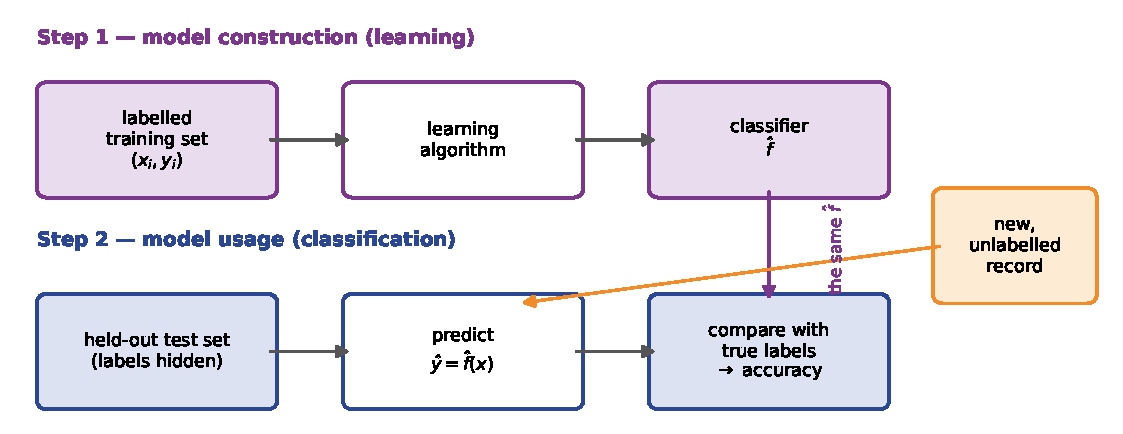
\includegraphics[width=0.94\textwidth]{workflow.pdf}
\caption{The two-step general approach to classification (Han, Kamber and Pei
\S8.1). Step 1 learns $\hat{f}$ from labelled data. Step 2 uses the
\emph{same} $\hat{f}$ twice: once on held-out data whose labels we know, to
estimate accuracy, and then on genuinely new records whose labels we do not.}
\label{fig:workflow}
\end{figure}

Han, Kamber and Pei describe classification as a two-step process, and it is
worth learning in that form because the examination asks for it.

\begin{enumerate}[leftmargin=*]
  \item \textbf{Model construction} (the learning step). A learning algorithm
    is given a training set of instances whose class labels are known, and
    produces a classifier. Because the labels are supplied, this is
    \emph{supervised} learning. The classifier can be a set of rules, a tree, a
    formula, a set of weights --- or, as we shall see, nothing at all.
  \item \textbf{Model usage} (the classification step). The classifier labels
    new instances. Before we trust it we estimate its accuracy on a
    \textbf{test set}: instances with known labels that were not used in step
    1. If the accuracy is acceptable, the classifier is applied to genuinely
    unlabelled records.
\end{enumerate}

The test set must be independent of the training set, for exactly the reason
the preprocessing unit gave: a model that has seen an instance can recite its
label, and reciting is not predicting. Section~\ref{sec:memorise} makes that
point in its sharpest possible form.

\subsection{The workflow in code}

Three lines is the whole of it. Fit, predict, evaluate.

\begin{lstlisting}
from sklearn.model_selection import train_test_split
from sklearn.neighbors import KNeighborsClassifier
from sklearn.metrics import accuracy_score, confusion_matrix

X, y = iris.data, iris.target
Xtr, Xte, ytr, yte = train_test_split(X, y, test_size=0.3,
                                      random_state=0, stratify=y)
print("training set", Xtr.shape, " test set", Xte.shape)

clf = KNeighborsClassifier(n_neighbors=3)   # step 1: model construction
clf.fit(Xtr, ytr)
pred = clf.predict(Xte)                     # step 2: model usage
print("first ten predictions", pred[:10])
print("first ten true labels", yte[:10])
print("test accuracy %.4f" % accuracy_score(yte, pred))
print(confusion_matrix(yte, pred))
\end{lstlisting}
\begin{codeout}
training set (105, 4)  test set (45, 4)
first ten predictions [2 2 0 0 1 0 1 2 0 1]
first ten true labels [2 2 0 0 1 0 1 2 0 1]
test accuracy 1.0000
confusion matrix (rows = true, cols = predicted)
[[15  0  0]
 [ 0 15  0]
 [ 0  0 15]]
\end{codeout}

Forty-five out of forty-five, and a confusion matrix with nothing off the
diagonal. Resist the urge to be pleased. \textbf{That is not a result, it is a
small sample.} Iris is an easy three-class problem and $45$ test rows are few
enough that a clean sweep is unremarkable; a different seed would give a
different number, and a confusion matrix of zeros teaches you nothing about
reading one.

So do it properly. Score the same classifier on \emph{all} $150$ rows, each
one predicted by a model that never saw it, using five-fold
cross-validation.

\begin{lstlisting}
from sklearn.model_selection import cross_val_predict, StratifiedKFold
CV = StratifiedKFold(5, shuffle=True, random_state=0)   # the one seed
cvp = cross_val_predict(KNeighborsClassifier(3), X, y, cv=CV)
print("accuracy %.4f" % accuracy_score(y, cvp))
print(confusion_matrix(y, cvp))
\end{lstlisting}
\begin{codeout}
5-fold cross-validated predictions for all 150 rows
accuracy 0.9600
confusion matrix (rows = true, cols = predicted)
[[50  0  0]
 [ 0 47  3]
 [ 0  3 47]]
\end{codeout}

Now the matrix says something the accuracy cannot. Every \emph{setosa} was
found --- the first row and first column are clean, because \emph{setosa} is
linearly separable from the other two and always has been. All six errors are
between \emph{versicolor} and \emph{virginica}: three each way. The single
number $0.9600$ hides \emph{which} mistake was made, and in a medical or
credit application it is the identity of the mistake that matters.

\begin{lstlisting}
from sklearn.metrics import classification_report
print(classification_report(y, cvp,
                            target_names=iris.target_names, digits=3))
\end{lstlisting}
\begin{codeout}
              precision    recall  f1-score   support

      setosa      1.000     1.000     1.000        50
  versicolor      0.940     0.940     0.940        50
   virginica      0.940     0.940     0.940        50

    accuracy                          0.960       150
   macro avg      0.960     0.960     0.960       150
weighted avg      0.960     0.960     0.960       150
\end{codeout}

\emph{Recall} for \emph{versicolor} is $47/50 = 0.940$: of the flowers that
really were \emph{versicolor}, we found $94\%$. \emph{Precision} for
\emph{versicolor} is also $47/50$, because exactly as many were wrongly
\emph{called} versicolor as were wrongly missed --- the errors happen to
balance here, and they usually do not. A later lecture in this unit builds the
full evaluation apparatus, ROC and AUC included; for now, always look at the
matrix as well as the number, and never read a confusion matrix off
forty-five rows if you can afford to cross-validate.

\subsection{The families of classification algorithm}
\label{sec:families}

Unit VI works through the main families. It is worth seeing the map before
walking the route.

\begin{center}\small
\begin{tabular}{@{}llp{6.1cm}@{}}
\toprule
\textbf{Family} & \textbf{Example} & \textbf{How it draws the boundary}\\
\midrule
instance-based & $k$-nearest neighbour & the training points themselves
  define it; no formula \emph{(this lecture)}\\
linear & logistic regression, linear SVM & one hyperplane
  $w^{\!\top}x + b = 0$\\
tree-based & ID3, CART & recursive axis-parallel splits\\
probabilistic & na\"ive Bayes & where the posterior probabilities are equal\\
kernel & SVM with an RBF kernel & a hyperplane in a transformed space\\
ensemble & bagging, boosting, random forest & many boundaries, combined
  by vote\\
neural & multi-layer perceptron & composed non-linear maps\\
\bottomrule
\end{tabular}
\end{center}

The two-step framing lets us compare them on the same footing, and the
one-dataset comparison below is a preview of the whole unit. Note the last
row: a \texttt{DummyClassifier} that always answers with the commonest class.
It is not a classifier so much as a ruler --- \textbf{every accuracy you quote
should be read against it}.

\begin{lstlisting}
from sklearn.pipeline import make_pipeline
from sklearn.preprocessing import StandardScaler
from sklearn.model_selection import StratifiedKFold, cross_val_score
CV = StratifiedKFold(5, shuffle=True, random_state=0)
for nm, mdl in [...]:                       # six classifiers
    s = cross_val_score(make_pipeline(StandardScaler(), mdl),
                        bc.data, bc.target, cv=CV)
    print("%-26s %10.4f %8.4f" % (nm, s.mean(), s.std()))
\end{lstlisting}
\begin{codeout}
classifier                     CV acc      std
KNeighborsClassifier(5)        0.9649   0.0215
LogisticRegression             0.9789   0.0142
GaussianNB                     0.9297   0.0124
DecisionTreeClassifier         0.9262   0.0218
SVC(rbf)                       0.9771   0.0070
DummyClassifier                0.6274   0.0039
\end{codeout}

\begin{figure}[htbp]
\centering
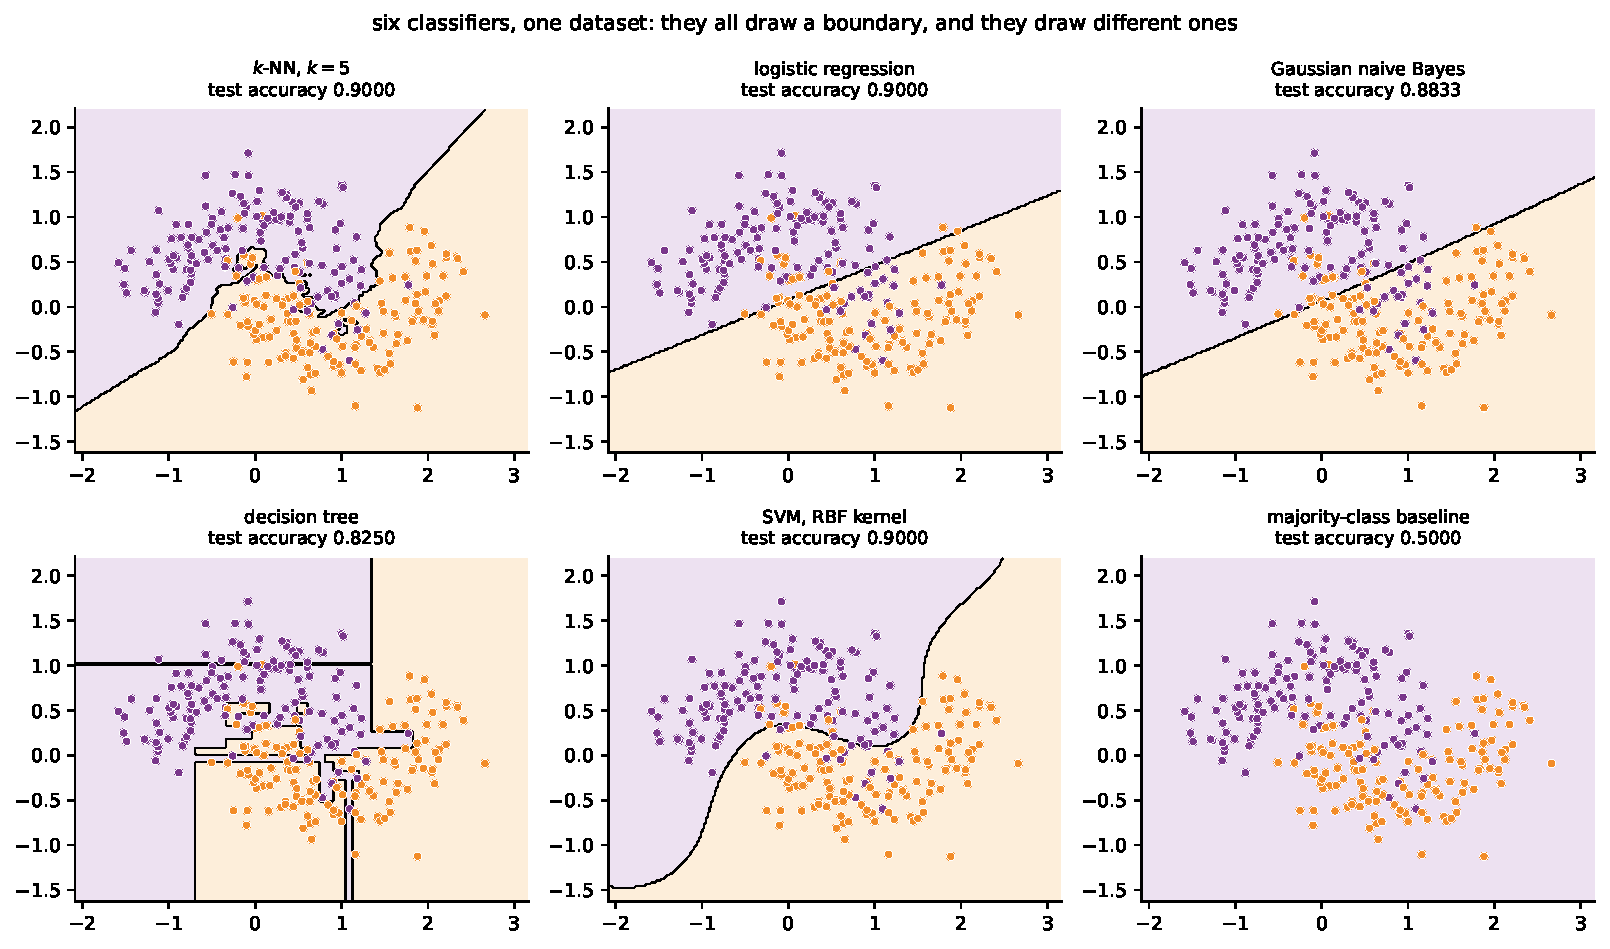
\includegraphics[width=0.92\textwidth]{classifier-landscape.pdf}
\caption{Six classifiers on the same 280 training points. Every one of them
partitions the plane; they disagree about how. $k$-NN follows the data,
logistic regression insists on a straight line, the tree can only cut parallel
to the axes, and the baseline paints the whole plane one colour.}
\label{fig:landscape}
\end{figure}

Two honest observations about that table. Nothing beats logistic regression on
this dataset, and $k$-NN is a full percentage point behind it. And the spread
between the five real classifiers is smaller than the gap between any of them
and the baseline. \textbf{Choosing the algorithm is usually a smaller decision
than people expect; choosing the features is usually a larger one.}

\subsection{Eager and lazy learners}
\label{sec:eagerlazy}

The single distinction that organises this lecture:

\begin{keyidea}
An \textbf{eager} learner does its work at training time: it digests the data
into a model and then throws the data away. A \textbf{lazy} learner does no
work at training time: it stores the data and defers everything until a
prediction is demanded.
\end{keyidea}

Logistic regression is eager. Fitting it means running an optimiser until a
weight vector converges; afterwards, the training rows can be deleted and the
model is unaffected. Decision trees, na\"ive Bayes, SVMs and neural networks
are all eager in the same sense.

$k$-nearest neighbour is lazy. ``Fitting'' it means keeping the table. All of
the work happens when you ask it a question, and the work is redone in full for
every question. Lazy learners are also called \textbf{instance-based} or
\textbf{memory-based} learners, and sometimes \emph{non-parametric}: there is
no fixed set of parameters whose number is decided in advance.

\begin{center}\small
\begin{tabular}{@{}lll@{}}
\toprule
 & \textbf{Eager} & \textbf{Lazy}\\
\midrule
training cost & high & essentially zero\\
prediction cost & low & high, and grows with $n$\\
memory after training & the model only & the whole training set\\
what it commits to & one global model & nothing until asked\\
new training data & usually refit from scratch & append the rows\\
examples & logistic regression, trees, SVM & $k$-NN, kernel regression\\
\bottomrule
\end{tabular}
\end{center}

The last-but-one row is a real advantage and is easy to overlook. A lazy
learner incorporates a new labelled example by adding a row. An eager learner
generally has to be refitted.

% =========================================================================
\section{Instance-based learning, measured}
\label{sec:lazy}

Assertions about cost are cheap. Here is the measurement, on
\texttt{load\_digits}: $1257$ training rows, $540$ test rows, $64$ features.

\begin{lstlisting}
import time
def timeit(f, reps=5):
    best = float("inf")
    for _ in range(reps):
        t0 = time.perf_counter(); f()
        best = min(best, time.perf_counter() - t0)
    return best

for name, model in [("KNeighborsClassifier(5)", KNeighborsClassifier(5)),
                    ("LogisticRegression", LogisticRegression(max_iter=5000)),
                    ("DecisionTreeClassifier", DecisionTreeClassifier(random_state=0)),
                    ("GaussianNB", GaussianNB())]:
    tf = timeit(lambda m=model: m.fit(Xdtr, ydtr))
    model.fit(Xdtr, ydtr)
    tp = timeit(lambda m=model: m.predict(Xdte))
    print(name, tf * 1e3, tp * 1e3, tp / tf,
          accuracy_score(ydte, model.predict(Xdte)))
\end{lstlisting}
\begin{codeout}
digits: 1257 training rows, 540 test rows, 64 features
model                      fit (ms)   pred (ms)   pred/fit      acc
KNeighborsClassifier(5)       0.234       3.077    13.1455   0.9796
LogisticRegression          844.267       0.101     0.0001   0.9611
DecisionTreeClassifier       10.019       0.079     0.0079   0.8426
GaussianNB                    0.856       0.749     0.8744   0.8481
\end{codeout}

\begin{caution}[The milliseconds above are the one thing a seed cannot fix]
Every other number in these notes is reproducible: fixed dataset, one seed,
same answer on your machine as on mine. \textbf{Timings are not.} They depend
on your processor, your BLAS build and whatever else is running, and repeated
runs on \emph{this} machine moved the $k$-NN \texttt{pred/fit} ratio between
about $11$ and $14$ for the same comparison.

So never quote a timing as a fact. State the cost claim in operation counts,
which are exact everywhere, and report the milliseconds separately as what
they are --- one measurement, on one machine, on one afternoon.
\end{caution}

Here are the counts, and they are the claim.

\begin{codeout}
  KNN  predict: 540 x 1257 distances x 64 features = 43441920 coordinate ops
  KNN  fit    : 0 distances -- it copies 80448 numbers and stops
  LR   predict: 540 x 10 classes x 64 features = 345600 multiply-adds
  LR   fit    : 172 L-BFGS iterations over all 1257 training rows
\end{codeout}

$k$-NN's \texttt{fit} performs \emph{no} distance computations at all: it
copies $80{,}448$ numbers and stops. Its \texttt{predict} performs
$540 \times 1257 = 678{,}780$ distance evaluations over $64$ coordinates each
--- $43{,}441{,}920$ coordinate operations. Logistic regression is the mirror
image: its \texttt{fit} runs $172$ L-BFGS iterations over all $1257$ rows,
and its \texttt{predict} is one $540\times64$ by $64\times10$ matrix product,
$345{,}600$ multiply--adds. Per prediction, $k$-NN does
$\mathbf{125.7}$ times as much arithmetic as logistic regression, on every
machine ever built.

The \texttt{pred/fit} column illustrates the same asymmetry with a clock on
it. For $k$-NN it is above one --- predicting costs more than fitting. For
logistic regression it is $0.0001$ --- predicting costs one ten-thousandth of
what fitting costs. Those two differ by about $10^5$, and that is the whole of
Section~\ref{sec:eagerlazy} in one comparison. Quote the ratio and the
counts; never the milliseconds.

\begin{figure}[htbp]
\centering
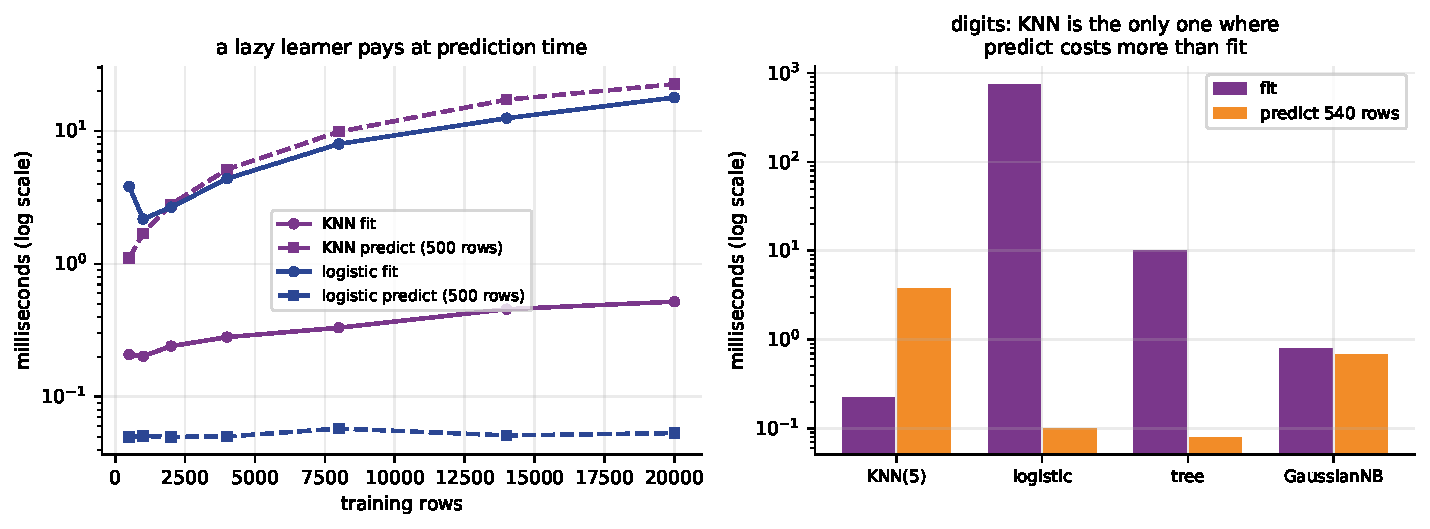
\includegraphics[width=0.94\textwidth]{lazy-vs-eager.pdf}
\caption{Left: as the training set grows from $500$ to $20{,}000$ rows,
$k$-NN's fit time stays flat and its prediction time grows linearly, while
logistic regression's fit time grows and its prediction time does not move.
Right: the same contrast on \texttt{digits}, on a log scale.}
\label{fig:lazy}
\end{figure}

\begin{worked}[Where does the time go?]
$k$-NN's \texttt{fit} does one thing: it copies the training matrix and, if
asked, builds an index over it. Its \texttt{predict} must, for every query
row, compute the distance to every stored row. With $n$ training rows, $m$
query rows and $d$ features that is $O(nmd)$ arithmetic operations. Doubling
the training set doubles the prediction time --- which is exactly what the left
panel of Figure~\ref{fig:lazy} shows.
\end{worked}

\begin{lstlisting}
Xbig, ybig = make_classification(n_samples=20000, n_features=20,
                                 n_informative=10, random_state=0)
Xq = Xbig[:500]                      # always predict the same 500 rows
for n in (500, 2000, 8000, 20000):
    ...                              # time fit and predict for each n
\end{lstlisting}
\begin{codeout}
train rows   KNN fit (ms)   KNN predict (ms)   LR fit (ms)   LR pred (ms)   KNN distances
       500          0.206              1.016         2.662         0.061          250000
      2000          0.237              2.702         2.700         0.049         1000000
      8000          0.295              9.921        10.945         0.058         4000000
     20000          0.523             22.039        17.430         0.045       10000000
\end{codeout}

The last column is the one to quote. Forty times the training rows is
\emph{exactly} forty times the distance computations --- $10{,}000{,}000$
against $250{,}000$ --- because every one of the $500$ query rows must be
compared with every stored row. That is arithmetic, and it is true on your
laptop, on mine and on a supercomputer.

The measured time grew by rather less than forty, and by a different factor
each time this was run. The shortfall is vectorisation: a bigger distance
matrix keeps the BLAS kernel busier per row, so the cost per distance falls
even as the number of distances rises. That is a property of the machine, not
of the algorithm. Logistic regression's prediction time did not move at all,
because its prediction does not involve the training rows in any way.

\subsection{And it has to keep the data}

\begin{lstlisting}
kn = KNeighborsClassifier(5).fit(Xdtr, ydtr)
print("stored training matrix shape", kn._fit_X.shape)
print("bytes of training data held  ", kn._fit_X.nbytes)
lr = LogisticRegression(max_iter=5000).fit(Xdtr, ydtr)
print("logistic regression stores   ",
      lr.coef_.nbytes + lr.intercept_.nbytes, "bytes")
\end{lstlisting}
\begin{codeout}
stored training matrix shape (1257, 64)
bytes of training data held   643584
logistic regression stores    5200 bytes, coef_ shape (10, 64)
ratio 123.8 x
\end{codeout}

A fitted $k$-NN on \texttt{digits} weighs $124$ times what a fitted logistic
regression weighs, and the ratio grows with the number of training rows while
the logistic model's size does not.

\begin{caution}[$k$-NN keeps your training data, and that is a privacy fact]
An eager model can be shipped without the data it was trained on. A $k$-NN
model \emph{is} the data. If the training rows are patient records or exam
scripts, deploying the classifier means deploying those records. This is not a
technicality --- it decides whether a model can leave the building.
\end{caution}

\subsection{Can an index rescue the prediction cost?}

Partly, and only in low dimensions. scikit-learn can build a KD-tree or a
ball-tree over the training points so that a query does not have to touch every
row. Here is that idea meeting Section~\ref{sec:curse} head-on.

\begin{lstlisting}
for d in (2, 10, 40):
    Xs, ys = make_classification(n_samples=5000, n_features=d, ...)
    for algo in ("brute", "kd_tree"):
        ...                              # time fit and predict
\end{lstlisting}
\begin{codeout}
features        algo     fit (ms)   predict (ms)
2              brute        0.314          9.055
2            kd_tree        1.489         15.361
2            kd_tree  subtrees pruned    6249   leaf visits    1500   leaves per query    1.5
10             brute        0.289         10.742
10           kd_tree        2.767         39.714
10           kd_tree  subtrees pruned   10056   leaf visits   28567   leaves per query   28.6
40             brute        0.287         16.707
40           kd_tree        6.931        169.059
40           kd_tree  subtrees pruned     127   leaf visits   63824   leaves per query   63.8
\end{codeout}

Ignore the milliseconds and read the pruning counts, which are exact and
identical on any machine. A KD-tree earns its keep by \emph{ruling regions
out}: at two features, a query descends to $1.5$ leaves on average and
$6249$ subtrees are discarded without being looked at. At ten features the
query already has to open $28.6$ leaves. At forty features only $127$
subtrees are pruned in a thousand queries and each query opens $63.8$
leaves --- essentially the whole tree.

That is the geometry of Section~\ref{sec:curse} arriving in a data
structure. If no region can be ruled out, the tree computes every distance
brute force would have computed \emph{and} pays for the traversal on top,
which is why the measured time is worse rather than better. Leave
\texttt{algorithm='auto'} alone; scikit-learn already knows this.

% =========================================================================
\section{$K$-nearest neighbour}
\label{sec:knn}

\subsection{The algorithm}

\begin{keyidea}
To classify a new instance $q$: measure the distance from $q$ to every training
instance, keep the $k$ closest, and return the commonest label among them.
That is the entire algorithm.
\end{keyidea}

Formally, given a training set $\mathcal{D} = \{(x_i, y_i)\}_{i=1}^{n}$, a
distance $d(\cdot,\cdot)$ and an integer $k$, let $N_k(q) \subseteq
\mathcal{D}$ be the $k$ instances with the smallest $d(q, x_i)$. Then

\[
  \hat{f}(q) \;=\; \arg\max_{c}\ \sum_{(x_i, y_i) \in N_k(q)}
  \mathbb{1}[y_i = c].
\]

The default distance is Euclidean:

\[
  d(p, q) \;=\; \sqrt{\sum_{j=1}^{d} (p_j - q_j)^2}.
\]

Two remarks before the arithmetic. First, ranking by $d$ and ranking by $d^2$
give the same order, because the square root is increasing --- so you may work
with squared distances throughout and take one square root at the end, or none
at all. Do this in the examination; it saves time and avoids errors. Second,
$k$ is not learned from the data. It is a \textbf{hyperparameter}, chosen by
validation, and Section~\ref{sec:k} is about choosing it.

\subsection{Worked by hand: seven points, one query}
\label{sec:hand}

\begin{worked}[1-NN on seven points]
A training set of seven instances with two features and two classes:

\begin{center}\small
\begin{tabular}{@{}lrrr@{}}
\toprule
point & $x_1$ & $x_2$ & class\\
\midrule
A & 1 & 1 & 0\\
B & 2 & 2 & 0\\
C & 1 & 3 & 0\\
D & 5 & 4 & 1\\
E & 6 & 5 & 1\\
F & 4 & 7 & 1\\
G & 6 & 2 & 0\\
\bottomrule
\end{tabular}
\end{center}

Classify $q_1 = (3, 3)$. Compute the squared distance to each point --- no
square roots yet:

\begin{center}\small
\begin{tabular}{@{}lccccccc@{}}
\toprule
point & A & B & C & D & E & F & G\\
\midrule
$(x_1-3)^2$ & 4 & 1 & 4 & 4 & 9 & 1 & 9\\
$(x_2-3)^2$ & 4 & 1 & 0 & 1 & 4 & 16 & 1\\
\midrule
$d^2$ & 8 & \textbf{2} & 4 & 5 & 13 & 17 & 10\\
$d$ & 2.8284 & \textbf{1.4142} & 2.0000 & 2.2361 & 3.6056 & 4.1231 & 3.1623\\
\bottomrule
\end{tabular}
\end{center}

Ranked nearest first: \textbf{B, C, D, A, G, E, F}. The nearest neighbour is
$B$, at $d = \sqrt{2} = 1.4142$, and $B$'s class is $\mathbf{0}$. So the 1-NN
prediction for $q_1$ is class $0$.
\end{worked}

Now the same thing in code, to see that the library does exactly that.

\begin{lstlisting}
Xh = np.array([[1,1],[2,2],[1,3],[5,4],[6,5],[4,7],[6,2]], dtype=float)
yh = np.array([0, 0, 0, 1, 1, 1, 0])
q1 = np.array([3.0, 3.0])

knn1 = KNeighborsClassifier(n_neighbors=1).fit(Xh, yh)
dist, idx = knn1.kneighbors(q1.reshape(1, -1))
print("sklearn nearest neighbour index", idx[0])
print("sklearn distance %.6f    by hand sqrt(2) = %.6f"
      % (dist[0][0], np.sqrt(2)))
print("sklearn prediction", knn1.predict(q1.reshape(1, -1))[0])
\end{lstlisting}
\begin{codeout}
sklearn nearest neighbour index [1] = point B
sklearn distance 1.414214    by hand sqrt(2) = 1.414214
sklearn prediction 0
\end{codeout}

Index $1$ is the second row, which is $B$. The distance agrees to six decimal
places with $\sqrt{2}$ worked out on paper. There is nothing in
\texttt{KNeighborsClassifier} that you did not just do by hand.

\begin{figure}[htbp]
\centering
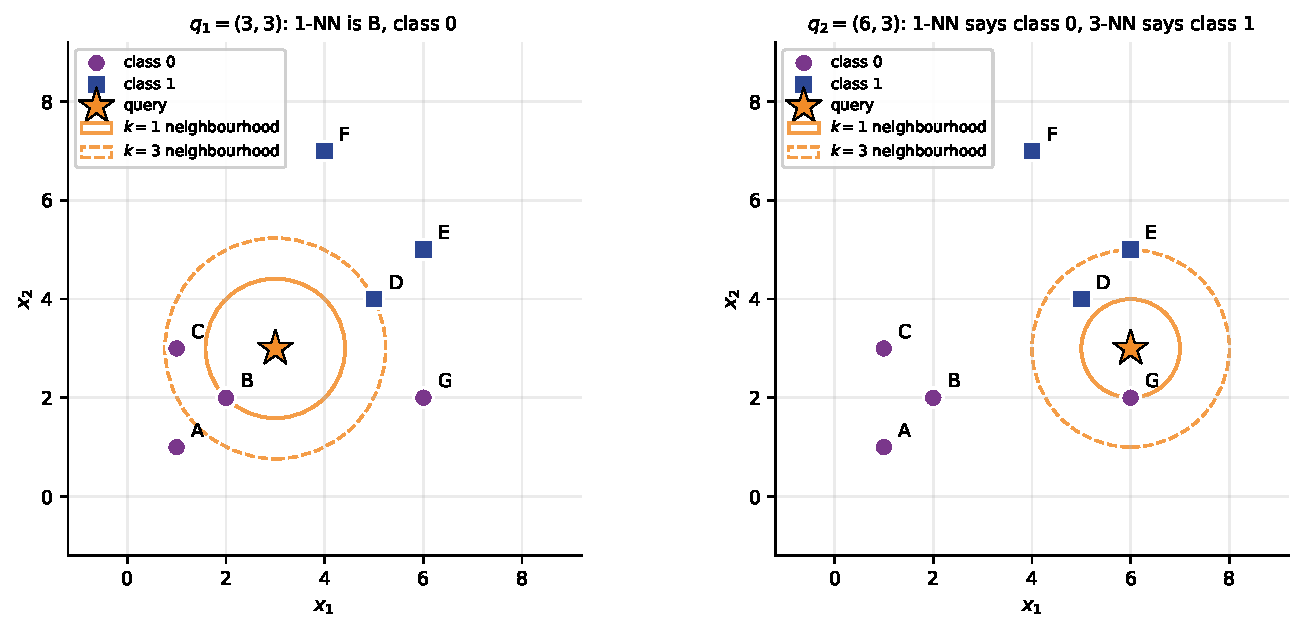
\includegraphics[width=0.94\textwidth]{hand-example.pdf}
\caption{The seven training points and the two queries of
Sections~\ref{sec:hand} and~\ref{sec:hand2}. The circles have radius equal to
the distance to the $1$st and $3$rd nearest neighbour, so what falls inside
each circle is exactly what votes.}
\label{fig:hand}
\end{figure}

\subsection{Worked by hand: the query where $k$ matters}
\label{sec:hand2}

Look again at point $G = (6,2)$. It is labelled class $0$, but it sits over on
the right among the class-$1$ points --- a mislabelled record, or a genuine but
unusual case. Now classify $q_2 = (6, 3)$, which lands right next to it.

\begin{worked}[$k$ changes the answer]
\begin{center}\small
\begin{tabular}{@{}lrrrr@{}}
\toprule
rank & point & $d^2$ & $d$ & class\\
\midrule
1 & G & 1 & 1.0000 & 0\\
2 & D & 2 & 1.4142 & 1\\
3 & E & 4 & 2.0000 & 1\\
4 & B & 17 & 4.1231 & 0\\
5 & F & 20 & 4.4721 & 1\\
6 & C & 25 & 5.0000 & 0\\
7 & A & 29 & 5.3852 & 0\\
\bottomrule
\end{tabular}
\end{center}

\begin{itemize}[leftmargin=*]
  \item $k=1$: neighbour $\{G\}$. Votes $0{:}1$, $1{:}0$. \textbf{Predict 0.}
  \item $k=3$: $\{G, D, E\}$. Votes $0{:}1$, $1{:}2$. \textbf{Predict 1.}
  \item $k=5$: $\{G, D, E, B, F\}$. Votes $0{:}2$, $1{:}3$. \textbf{Predict 1.}
  \item $k=7$: everything. Votes $0{:}4$, $1{:}3$. \textbf{Predict 0.}
\end{itemize}
\end{worked}

\begin{lstlisting}
for k in (1, 3, 5, 7):
    m = KNeighborsClassifier(n_neighbors=k).fit(Xh, yh)
    votes = np.bincount(yh[ob[:k]], minlength=2)
    print("k=%d  votes  class0=%d  class1=%d  ->  predict %d   (sklearn %d)"
          % (k, votes[0], votes[1], votes.argmax(),
             m.predict(q2.reshape(1, -1))[0]))
\end{lstlisting}
\begin{codeout}
k=1  votes  class0=1  class1=0  ->  predict 0   (sklearn 0)
k=3  votes  class0=1  class1=2  ->  predict 1   (sklearn 1)
k=5  votes  class0=2  class1=3  ->  predict 1   (sklearn 1)
k=7  votes  class0=4  class1=3  ->  predict 0   (sklearn 0)
\end{codeout}

Three lessons in one table. At $k=1$ a single odd training point dictates the
answer. At $k=3$ and $k=5$ the vote overrules it, which is what averaging is
for. At $k=7$ --- which is $n$, the whole training set --- the classifier has
stopped looking at $q_2$ at all and simply returns the commonest label in the
data. \textbf{At $k = n$, $k$-NN is the majority-class baseline.}

\subsection{1-NN is a Voronoi tessellation}

There is a clean geometric description of the $k=1$ classifier. Each training
point owns the region of space closer to it than to any other training point.
Those regions are \textbf{Voronoi cells}, and 1-NN labels a query with the
label of whichever cell it falls in. The decision boundary is what remains
after erasing the walls between adjacent cells of the same label.

\begin{figure}[htbp]
\centering
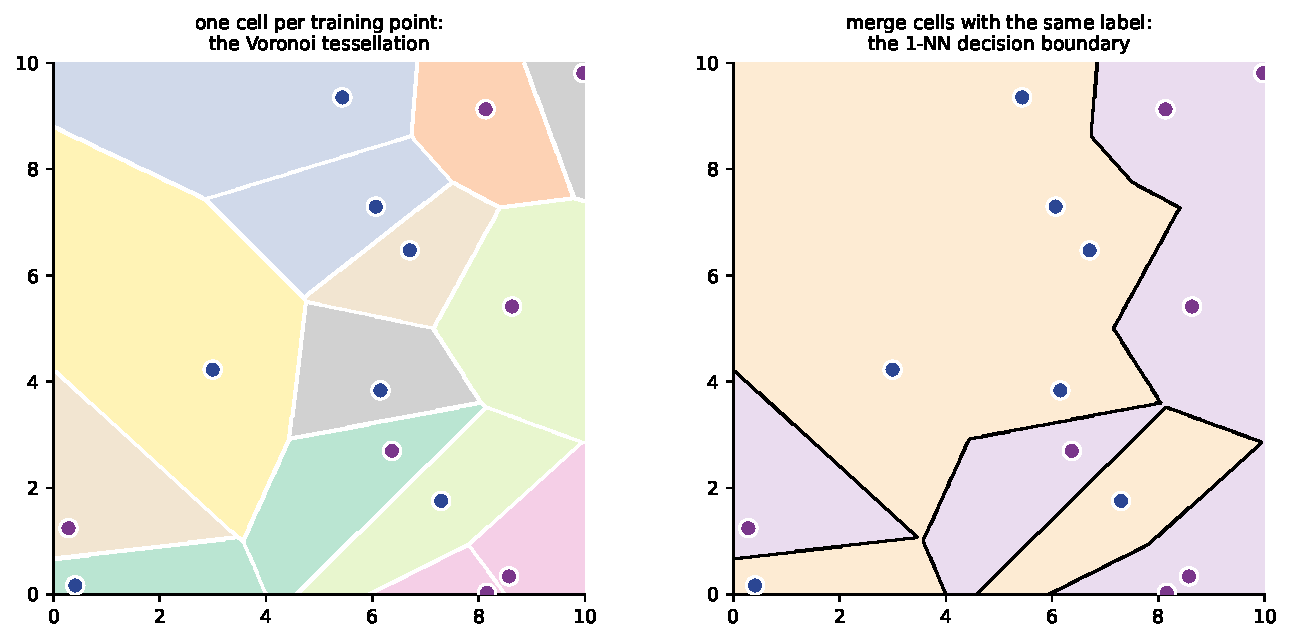
\includegraphics[width=0.86\textwidth]{voronoi.pdf}
\caption{Left: fourteen training points and their Voronoi cells --- one cell
per point, containing everything closer to it than to any other. Right: colour
each cell by its point's label and erase the internal walls. That is the 1-NN
decision boundary, and it is jagged because it is made of perpendicular
bisectors between individual data points.}
\label{fig:voronoi}
\end{figure}

Two things follow from the picture, and they are the reason
Section~\ref{sec:k} exists. The boundary passes exactly halfway between pairs
of opposite-labelled points, so \textbf{moving one training point moves the
boundary}; and every training point, however atypical, gets a cell of its own.

% =========================================================================
\section{Choosing $k$}
\label{sec:k}

\subsection{$k=1$ memorises, and here is the proof}
\label{sec:memorise}

\begin{keyidea}
A 1-NN classifier scores exactly $1.0$ on its own training set, always, on
every dataset, regardless of how much noise is in it. The reason is trivial and
the consequence is not: \textbf{training accuracy tells you nothing about a
$k$-NN model}.
\end{keyidea}

Ask 1-NN about a row that is in the training set. The nearest training point to
that row is the row itself, at distance $0$. Its label is the true label. So
the prediction is correct. Every time.

\begin{lstlisting}
m1 = KNeighborsClassifier(1).fit(Xbtr_s, ybtr)
dist, idx = m1.kneighbors(Xbtr_s[:5])
for i in range(5):
    print("  row %d -> training row %d at distance %.6f"
          % (i, idx[i][0], dist[i][0]))
print("every training row is its own nearest neighbour:",
      bool(np.all(m1.kneighbors(Xbtr_s)[1][:, 0] == np.arange(len(Xbtr_s)))))
print("training accuracy at k=1: %.6f" % m1.score(Xbtr_s, ybtr))
\end{lstlisting}
\begin{codeout}
nearest neighbour of the first five training rows:
  row 0 -> training row 0 at distance 0.000000
  row 1 -> training row 1 at distance 0.000000
  row 2 -> training row 2 at distance 0.000000
  row 3 -> training row 3 at distance 0.000000
  row 4 -> training row 4 at distance 0.000000
every training row is its own nearest neighbour: True
training accuracy at k=1: 1.000000
\end{codeout}

\begin{caution}[``My model got 100\% accuracy''] % chktex 36
Every year somebody reports a perfect $k$-NN score and is delighted. Check
which set it was measured on. A training accuracy of $1.0$ at $k=1$ is a
consequence of arithmetic, not of learning, and it is compatible with the model
being useless. Quote a cross-validated score or a held-out score, always.
\end{caution}

\subsection{The gap between training and test accuracy}

\begin{lstlisting}
Xbtr, Xbte, ybtr, ybte = train_test_split(bc.data, bc.target, test_size=0.3,
                                          random_state=0, stratify=bc.target)
sc = StandardScaler().fit(Xbtr)
Xbtr_s, Xbte_s = sc.transform(Xbtr), sc.transform(Xbte)
for k in (1, 3, 5, 11, 25, 51, 101, 199):
    m = KNeighborsClassifier(k).fit(Xbtr_s, ybtr)
    print(k, m.score(Xbtr_s, ybtr), m.score(Xbte_s, ybte))
\end{lstlisting}
\begin{codeout}
   k   train acc   test acc      gap
   1      1.0000     0.9474    +0.0526
   3      0.9899     0.9415    +0.0484
   5      0.9799     0.9474    +0.0325
  11      0.9774     0.9357    +0.0417
  25      0.9598     0.9415    +0.0183
  51      0.9523     0.9474    +0.0049
 101      0.9271     0.9181    +0.0090
 199      0.8643     0.8538    +0.0105
\end{codeout}

The \texttt{gap} column shrinks monotonically in spirit as $k$ grows: $+0.0526$
at $k=1$, $+0.0049$ at $k=51$. A large gap between training and test accuracy
is the signature of \textbf{over-fitting}, and in $k$-NN over-fitting is
controlled entirely by $k$.

\subsection{What $k$ does to the boundary}

\begin{figure}[htbp]
\centering
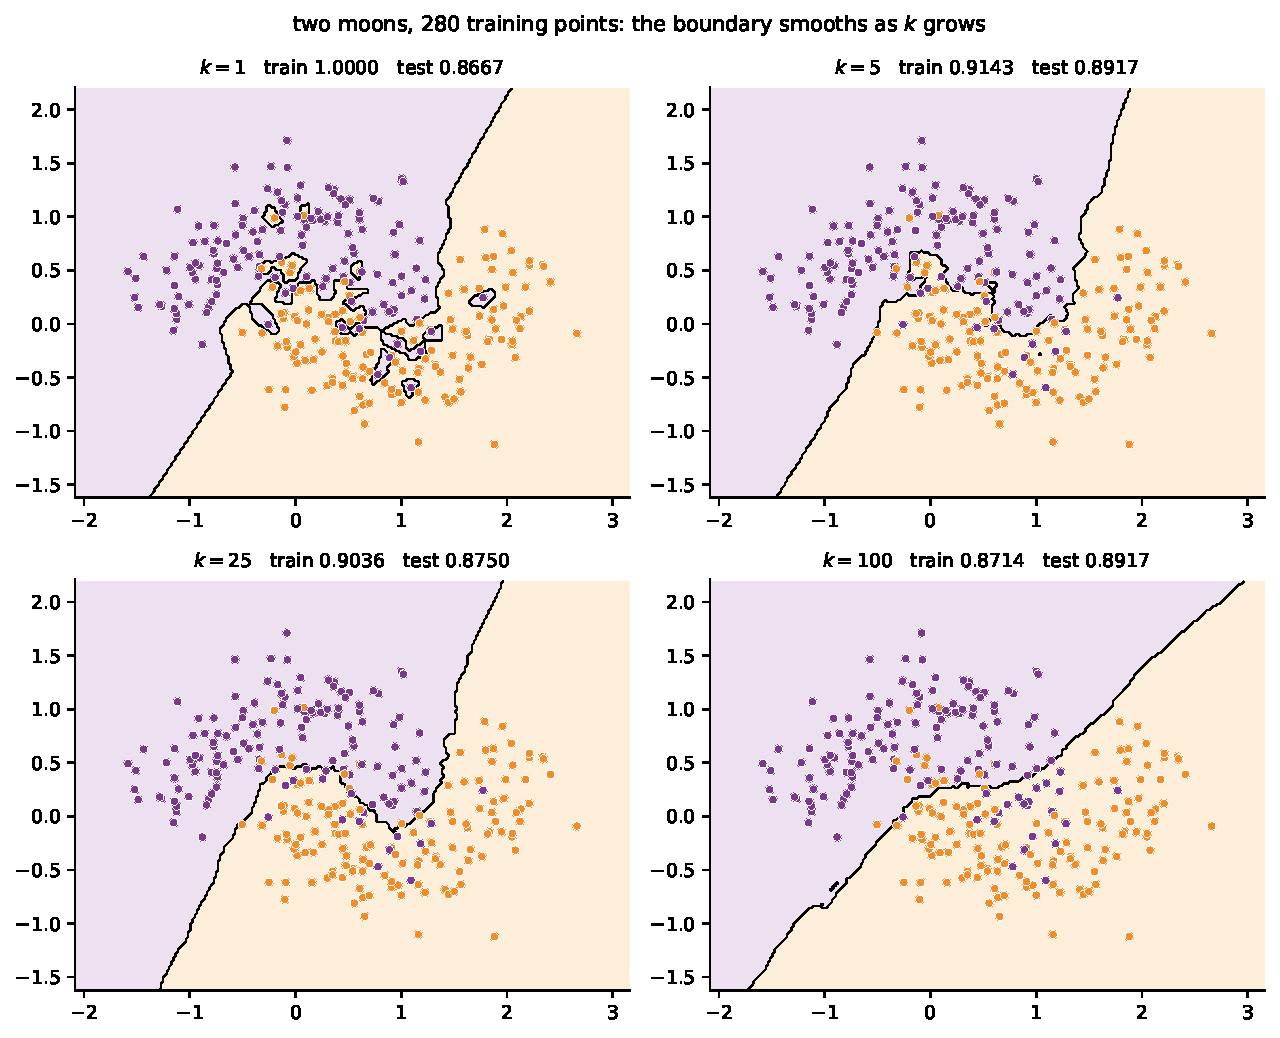
\includegraphics[width=0.80\textwidth]{k-boundaries.pdf}
\caption{The same 280 training points at four values of $k$. At $k=1$ the
boundary wraps around every individual point and the training accuracy is
$1.0000$; at $k=100$ it is nearly a straight line. Note that the test accuracy
across these four panels varies by only about one and a half points --- the
boundary changes far more dramatically than the score does.}
\label{fig:kbound}
\end{figure}

The progression in Figure~\ref{fig:kbound} is the whole story of $k$:

\begin{itemize}[leftmargin=*]
  \item \textbf{Small $k$: low bias, high variance.} The model makes very few
    assumptions and will fit any shape --- including the shape of the noise. Move
    one training point and the boundary moves.
  \item \textbf{Large $k$: high bias, low variance.} The model averages over a
    wide neighbourhood and produces a smooth, stable boundary that may be too
    smooth to capture the real structure.
  \item \textbf{$k = n$:} the majority-class baseline, as we proved by hand in
    Section~\ref{sec:hand2}.
\end{itemize}

A useful rule of thumb for reasoning about this: the effective number of
``parameters'' of a $k$-NN model is roughly $n/k$, because the training set is
effectively divided into $n/k$ neighbourhoods each producing one answer. At
$k=1$ that is $n$ parameters for $n$ data points, which is the definition of
memorising.

\subsection{The validation curve}

\begin{figure}[htbp]
\centering
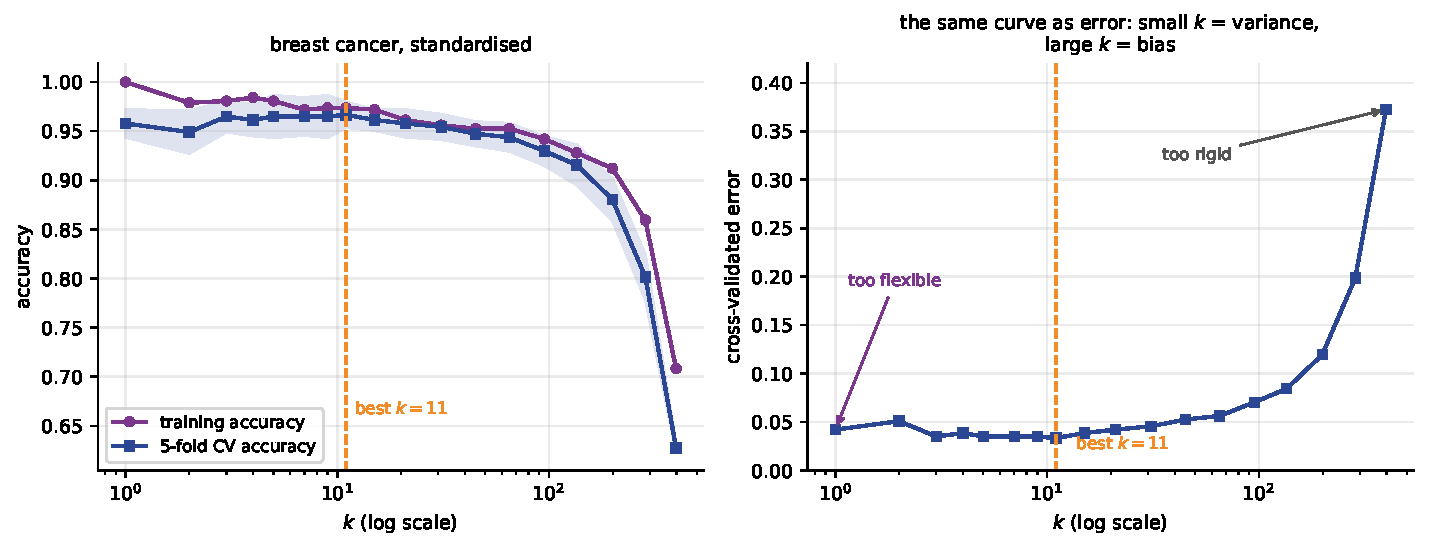
\includegraphics[width=0.94\textwidth]{k-curve.pdf}
\caption{Left: training and 5-fold cross-validated accuracy against $k$ on
standardised \texttt{breast\_cancer}. Right: the same cross-validated numbers
plotted as error, which is the familiar U shape. Both ends are bad, for
opposite reasons.}
\label{fig:kcurve}
\end{figure}

\begin{lstlisting}
for k in [1, 2, 3, 5, 7, 9, 11, 15, 21, 31, 45, 65, 95, 135, 199, 285, 398]:
    pipe = make_pipeline(StandardScaler(), KNeighborsClassifier(k))
    s = cross_val_score(pipe, bc.data, bc.target, cv=CV)
    print("%4d      %.4f          %.4f" % (k, s.mean(), s.std()))
\end{lstlisting}
\begin{codeout}
   k    5-fold CV accuracy      std
   1          0.9578          0.0140
   2          0.9491          0.0217
   3          0.9649          0.0157
   5          0.9649          0.0215
   7          0.9649          0.0192
   9          0.9649          0.0215
  11          0.9666          0.0129
  15          0.9613          0.0106
  21          0.9578          0.0140
  31          0.9543          0.0128
  45          0.9473          0.0123
  65          0.9438          0.0142
  95          0.9297          0.0146
 135          0.9156          0.0204
 199          0.8805          0.0211
 285          0.8015          0.0229
 398          0.6274          0.0039
best k = 11 at CV accuracy 0.9666
majority-class baseline 0.6274
\end{codeout}

Three things to read off honestly.

\begin{enumerate}[leftmargin=*]
  \item The best $k$ is $11$, at $0.9666$. The curve rises from $0.9578$ at
    $k=1$, peaks, and then falls away steadily.
  \item The peak is \textbf{shallow}. Everything from $k=3$ to $k=15$ is within
    one standard deviation of the best. Do not report ``the optimal $k$ is
    $11$'' as though $9$ were meaningfully worse; report the plateau.
  \item At $k=398$ --- which is $n$ minus the held-out fold --- the accuracy is
    $0.6274$, which is \emph{exactly} the majority-class baseline. The
    arithmetic of Section~\ref{sec:hand2} predicted that number before we ran
    anything.
\end{enumerate}

\begin{tryit}
Change the dataset in the loop above from \texttt{bc} to \texttt{wine} and run
it again. The peak moves, and the fall-off is much steeper, because
\texttt{wine} has $178$ rows to \texttt{breast\_cancer}'s $569$: with fewer
rows, $k=95$ is a far larger fraction of the data. \textbf{The right $k$
depends on $n$}, which is why there is no universal answer and why you must
cross-validate.
\end{tryit}

\begin{caution}[Choose $k$ inside the cross-validation, not outside it]
The loop above chose $k=11$ by looking at cross-validated scores on the whole
of \texttt{breast\_cancer}. If you now report $0.9666$ as your estimate of
future accuracy, that number is optimistic --- you selected $k$ using the same
folds you are quoting. Use \texttt{GridSearchCV} inside an outer
cross-validation, or hold out a genuinely untouched test set. This is the
selection-bias rule from the preprocessing unit, arriving in a new costume.
\end{caution}

% =========================================================================
\section{Scaling is not optional}
\label{sec:scale}

\subsection{The arithmetic, on one pair of patients}

$k$-NN's only input is a distance, and a distance is a sum over the columns.
If one column is measured in numbers a thousand times larger than another, its
squared differences are a million times larger, and it supplies essentially all
of the distance. The other columns are still there; they simply do not matter.

\begin{worked}[Two patients from \texttt{breast\_cancer}]
Take rows $0$ and $1$ of \texttt{load\_breast\_cancer}, and look at two of
their thirty columns:

\begin{center}\small
\begin{tabular}{@{}lrrrr@{}}
\toprule
feature & patient 0 & patient 1 & difference & (difference)$^2$\\
\midrule
mean area & $1001.0000$ & $1326.0000$ & $-325.0000$ & $105625.0000$\\
mean smoothness & $0.1184$ & $0.0847$ & $0.0337$ & $0.0011$\\
\bottomrule
\end{tabular}
\end{center}

The squared distance over all thirty columns is $116779.5720$. So
\emph{mean area} alone supplies $105625 / 116779.5720 = 90.45\%$ of it, and
\emph{mean smoothness} supplies $0.0011 / 116779.5720 \approx
0.000001\%$ --- one part in a hundred million.

Both are real medical measurements. Neither is more important than the other.
The only difference between them is the unit they happen to be recorded in.
\end{worked}

\begin{lstlisting}
p, q = bc.data[0], bc.data[1]
tot = ((p - q) ** 2).sum()
share = (p - q) ** 2 / tot
for j in np.argsort(share)[::-1][:4]:
    print("  %-24s contributes %8.4f%%" % (cols[j], 100 * share[j]))
\end{lstlisting}
\begin{codeout}
squared distance over all 30 features 116779.5720
  mean area                contributes  90.4482%
  area error               contributes   5.3876%
  worst area               contributes   3.3987%
  worst perimeter          contributes   0.5700%
the two area columns together contribute 93.8469%
the 27 columns that are not areas contribute 0.7655%
\end{codeout}

Three area columns supply $99.23\%$ of the distance; the other twenty-seven
measurements share $0.7655\%$ between them. \textbf{Unscaled $k$-NN on this
dataset is a classifier that uses three columns and ignores the rest.}

\subsection{It changes which point is nearest}

The share argument is suggestive. This is the demonstration.

\begin{lstlisting}
raw1 = KNeighborsClassifier(1).fit(Xbtr, ybtr)         # unscaled
std1 = KNeighborsClassifier(1).fit(Xbtr_s, ybtr)       # standardised
n_raw = raw1.kneighbors(Xbte, return_distance=False)[:, 0]
n_std = std1.kneighbors(Xbte_s, return_distance=False)[:, 0]
print("test rows whose nearest neighbour changes: %d of %d"
      % (int((n_raw != n_std).sum()), len(n_raw)))
\end{lstlisting}
\begin{codeout}
test rows whose nearest neighbour changes when we standardise: 164 of 171
of those, 19 change the predicted class
example: test row 5, true label 1
  raw          nearest is training row 206, label 0
  standardised nearest is training row 69, label 1
\end{codeout}

$164$ of $171$ test patients get a different nearest neighbour, and for $19$ of
them the \emph{answer} changes. Test row $5$ is genuinely class $1$;
standardising is what gets it right.

\begin{figure}[htbp]
\centering

\includegraphics[width=\textwidth]{scaling.pdf}
\caption{Left and centre: one held-out patient (star) and its nearest training
neighbour (circled), on two features, before and after standardising. The
neighbour changes and so does the predicted class. Right: what standardising is
worth to a $k=5$ classifier on four bundled datasets.}
\label{fig:scaling}
\end{figure}

\subsection{What it is worth, measured}

\begin{lstlisting}
for nm, d in [("iris", iris), ("wine", wine), ("breast_cancer", bc),
              ("digits", dg)]:
    a = cross_val_score(KNeighborsClassifier(5), d.data, d.target, cv=CV).mean()
    b = cross_val_score(make_pipeline(StandardScaler(),
                                      KNeighborsClassifier(5)),
                        d.data, d.target, cv=CV).mean()
    print("%-16s %10.4f %10.4f %+9.4f" % (nm, a, b, b - a))
\end{lstlisting}
\begin{codeout}
dataset                 raw     scaled      gain
iris                 0.9533     0.9533   +0.0000
wine                 0.6633     0.9608   +0.2975
breast_cancer        0.9315     0.9649   +0.0334
digits               0.9855     0.9766   -0.0089
feature std ratio (widest/narrowest column):
  iris                      4.1
  wine                   2530.3
  breast_cancer        215170.7
\end{codeout}

Read all four rows, including the two that do not support a simple slogan.

\begin{itemize}[leftmargin=*]
  \item \texttt{wine}: $+0.2975$. Thirty percentage points from four lines of
    preprocessing. Its widest column has a standard deviation $2530\times$ the
    narrowest --- \texttt{proline}, measured in the hundreds, against
    \texttt{hue}, measured around $1$.
  \item \texttt{breast\_cancer}: $+0.0334$, despite a std ratio of
    $215{,}171$. Larger ratio, smaller gain: the area columns that dominate the
    distance happen also to be genuinely informative, so ignoring the rest was
    not fatal. \textbf{The size of the scale disparity does not predict the
    size of the gain.}
  \item \texttt{iris}: $+0.0000$ to four decimal places. All four columns are
    centimetre measurements of the same flower, within a factor of $4$ of each
    other. There was nothing to fix.
  \item \texttt{digits}: $-0.0089$. Standardising made it \emph{worse}. Every
    one of the $64$ features is already a pixel intensity on the same $0$--$16$
    scale, so scaling had no disparity to correct --- but the border pixels are
    almost always $0$, and dividing an almost-constant column by its tiny
    standard deviation inflates its noise into a full-sized feature.
\end{itemize}

\begin{keyidea}
Scale when the columns are in different units. Do not scale reflexively when
they are already commensurable: standardising a near-constant column amplifies
its noise. On \texttt{digits} that cost $0.0089$ of accuracy.
\end{keyidea}

\begin{caution}[Fit the scaler on the training rows only]
\texttt{StandardScaler} learns a mean and a standard deviation. Those are
numbers learned from data, and the rule from the preprocessing unit applies
without change: learn them from the training split, apply them to the test
split. In practice, put the scaler and the classifier in a
\texttt{Pipeline} and let \texttt{cross\_val\_score} refit both inside every
fold, as every listing in these notes does.
\end{caution}

% =========================================================================
\section{Distance metrics and weighted voting}
\label{sec:metric}

\subsection{The Minkowski family}

Euclidean distance is one choice among many. The \textbf{Minkowski distance of
order $p$} is

\[
  d_p(a, b) \;=\; \Bigl( \sum_{j=1}^{d} |a_j - b_j|^{p} \Bigr)^{1/p},
  \qquad p \ge 1,
\]

and it contains the familiar metrics as special cases:

\begin{center}\small
\begin{tabular}{@{}llp{6.4cm}@{}}
\toprule
$p$ & name & character\\
\midrule
$1$ & Manhattan, city-block, $L_1$ & sum of the coordinate differences;
  robust to one large discrepancy\\
$2$ & Euclidean, $L_2$ & straight-line distance; the default\\
$p$ & Minkowski-$p$ & \texttt{KNeighborsClassifier(p=...)}\\
$\infty$ & Chebyshev, $L_\infty$ & the single largest coordinate difference\\
\bottomrule
\end{tabular}
\end{center}

The left panel of Figure~\ref{fig:metrics} draws the set of points at distance
exactly $1$ from the origin under each. A diamond for $p=1$, a circle for
$p=2$, a square for $p=\infty$. \textbf{Changing $p$ changes the shape of
``nearby''}, and therefore changes who your neighbours are.

\begin{figure}[htbp]
\centering
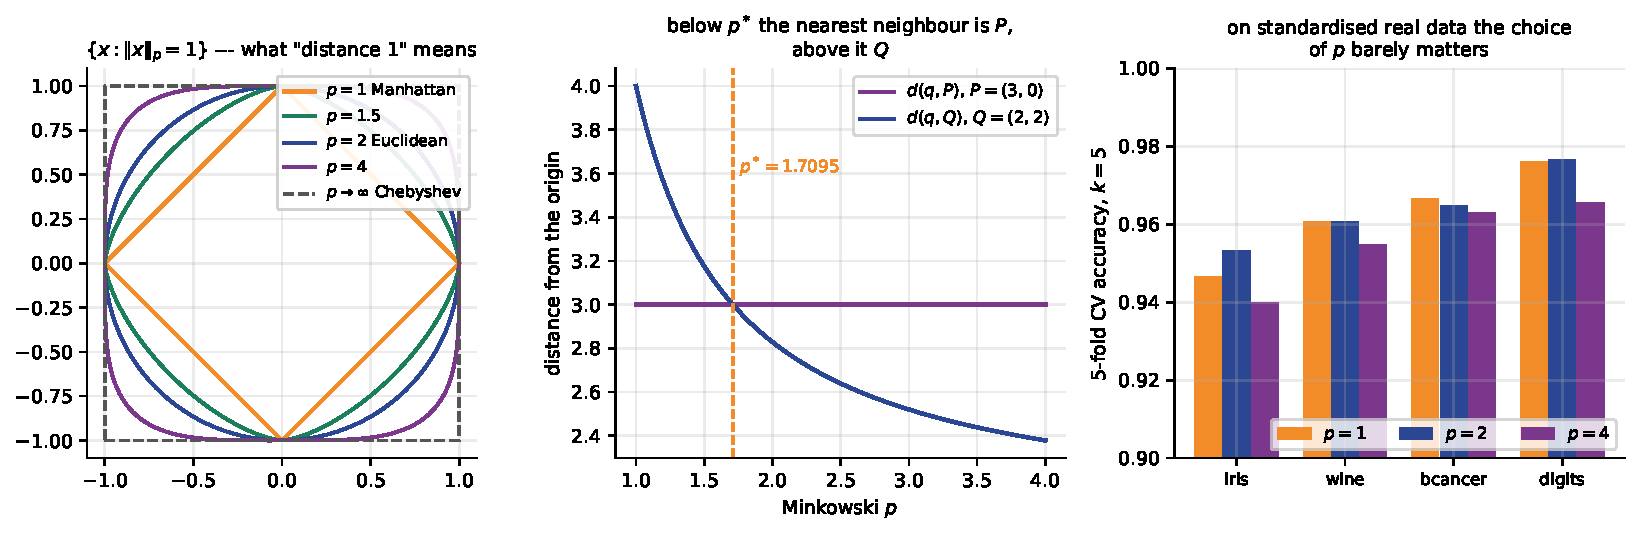
\includegraphics[width=\textwidth]{metrics.pdf}
\caption{Left: unit balls of the Minkowski family. Centre: the crossover of
Section~\ref{sec:crossover} --- below $p^\ast = 1.7095$ the nearest neighbour is
$P$, above it $Q$. Right: on standardised real data the choice of $p$ moves the
accuracy by well under a point.}
\label{fig:metrics}
\end{figure}

\subsection{Worked: where two metrics disagree}
\label{sec:crossover}

\begin{worked}[The same query, two answers]
Query $q = (0,0)$. Two candidate neighbours:
$P = (3, 0)$ of class $0$, and $Q = (2, 2)$ of class $1$.

\emph{Manhattan.} $d_1(q,P) = |3| + |0| = 3$. $d_1(q,Q) = |2| + |2| = 4$.
Nearest is $P$; predict class $0$.

\emph{Euclidean.} $d_2(q,P) = \sqrt{9} = 3$. $d_2(q,Q) = \sqrt{4+4} =
\sqrt{8} = 2.8284$. Nearest is $Q$; predict class $1$.

Same data, same $k$, opposite answers. Where does the switch happen? Set the
two Minkowski distances equal:
\[
  3 \;=\; \bigl(2^p + 2^p\bigr)^{1/p} \;=\; \bigl(2 \cdot 2^p\bigr)^{1/p}
    \;=\; 2^{\,1 + 1/p}.
\]
Take $\log_2$ of both sides: $\log_2 3 = 1 + 1/p$, so
\[
  p^\ast \;=\; \frac{1}{\log_2 3 - 1} \;=\; 1.709511.
\]
Below $p^\ast$ the answer is class $0$; above it, class $1$.
\end{worked}

\begin{lstlisting}
for pw in (1.0, 1.5, 1.70951, 2.0, 3.0, 10.0):
    dP = (np.abs(P) ** pw).sum() ** (1 / pw)
    dQ = (np.abs(Q) ** pw).sum() ** (1 / pw)
    print("p=%-8.5g  d(q,P)=%.4f   d(q,Q)=%.4f   nearest = %s"
          % (pw, dP, dQ, "P" if dP < dQ else "Q"))
\end{lstlisting}
\begin{codeout}
p=1         d(q,P)=3.0000   d(q,Q)=4.0000   nearest = P
p=1.5       d(q,P)=3.0000   d(q,Q)=3.1748   nearest = P
p=1.7095    d(q,P)=3.0000   d(q,Q)=3.0000   nearest = P
p=2         d(q,P)=3.0000   d(q,Q)=2.8284   nearest = Q
p=3         d(q,P)=3.0000   d(q,Q)=2.5198   nearest = Q
p=10        d(q,P)=3.0000   d(q,Q)=2.1435   nearest = Q
crossover: 3 = 2^(1+1/p)  gives  p = 1/(log2(3)-1) = 1.709511
Chebyshev (p -> inf): d(q,P)=3.0   d(q,Q)=2.0
\end{codeout}

\begin{lstlisting}
Xm = np.vstack([P, Q]); ym = np.array([0, 1])
for pw, nm in [(1, "manhattan"), (2, "euclidean")]:
    m = KNeighborsClassifier(1, p=pw).fit(Xm, ym)
    print("p=%d (%-9s) predicts class %d for the origin"
          % (pw, nm, m.predict(qm.reshape(1, -1))[0]))
\end{lstlisting}
\begin{codeout}
p=1 (manhattan) predicts class 0 for the origin
p=2 (euclidean) predicts class 1 for the origin
\end{codeout}

\begin{keyidea}
The distance metric is part of the model, not a detail of the implementation.
Two $k$-NN classifiers with the same $k$ and the same data are different
classifiers if their $p$ differs.
\end{keyidea}

\begin{figure}[htbp]
\centering
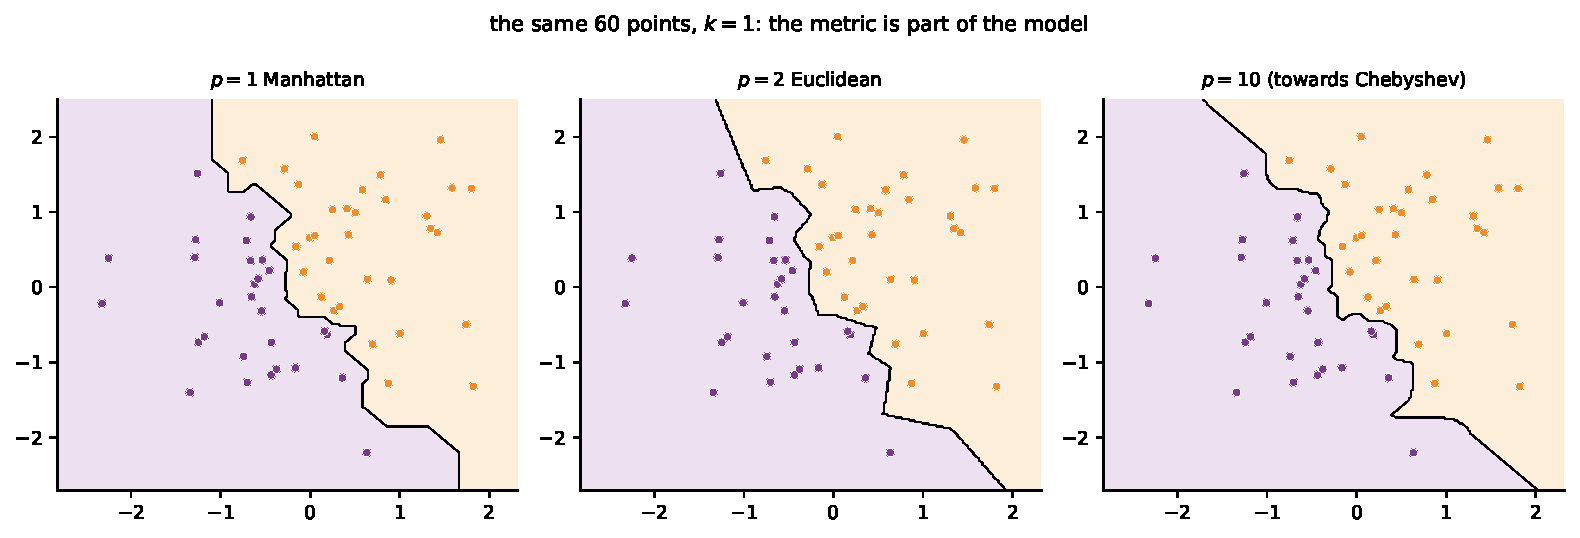
\includegraphics[width=0.94\textwidth]{metric-boundaries.pdf}
\caption{The same sixty points and the same $k=1$, under three metrics. The
Manhattan boundary is built from diagonal facets, the Euclidean one from
perpendicular bisectors, the near-Chebyshev one from axis-aligned steps.}
\label{fig:metricbound}
\end{figure}

\subsection{Does it matter in practice?}

\begin{lstlisting}
for nm, d in [("iris", iris), ("wine", wine), ("breast_cancer", bc),
              ("digits", dg)]:
    for pw in (1, 2, 4):
        pipe = make_pipeline(StandardScaler(), KNeighborsClassifier(5, p=pw))
        ...
\end{lstlisting}
\begin{codeout}
dataset                p=1       p=2       p=4   chebyshev
iris                0.9467    0.9533    0.9400      0.9400
wine                0.9606    0.9608    0.9549      0.9214
breast_cancer       0.9666    0.9649    0.9631      0.9420
digits              0.9761    0.9766    0.9655      0.9255
\end{codeout}

Honest answer: on these four standardised datasets, not much. $p=1$ and $p=2$
are within $0.002$ of each other everywhere; Chebyshev is consistently the
worst, by up to $0.05$ on \texttt{digits}, because throwing away all but the
single largest coordinate difference discards most of the information. Treat
$p$ as a hyperparameter worth one line in a grid search, not as the place where
your accuracy is hiding.

\subsection{Distance-weighted voting}

A plain vote treats the nearest neighbour and the $k$th-nearest as equals. That
is odd if one is right beside the query and the other is far away.
\textbf{Distance-weighted $k$-NN} gives each neighbour a vote of weight
$1/d$ (scikit-learn's \texttt{weights='distance'}).

\begin{worked}[Five neighbours, two answers]
The five nearest neighbours of a query, with their distances and labels:

\begin{center}\small
\begin{tabular}{@{}lrrrrr@{}}
\toprule
neighbour & $n_1$ & $n_2$ & $n_3$ & $n_4$ & $n_5$\\
\midrule
distance $d$ & $1$ & $2$ & $4$ & $4$ & $5$\\
label & 1 & 0 & 0 & 0 & 0\\
weight $1/d$ & $1.0000$ & $0.5000$ & $0.2500$ & $0.2500$ & $0.2000$\\
\bottomrule
\end{tabular}
\end{center}

\emph{Uniform vote:} class $0$ gets four votes, class $1$ gets one.
\textbf{Predict 0} --- comfortably.

\emph{Weighted vote:} class $1$ gets $1.0000$; class $0$ gets
$0.5 + 0.25 + 0.25 + 0.2 = 1.2000$. \textbf{Predict 0} --- but only just, and
the margin has collapsed from $4$:$1$ to $1.2$:$1.0$.

Move $n_1$ to $d = 0.8$ and its weight becomes $1.25$: the weighted vote flips
to class $1$ while the uniform vote is unchanged at $4$:$1$.
\end{worked}

\begin{codeout}
neighbour distances [1. 2. 4. 4. 5.]
neighbour labels    [1 0 0 0 0]
uniform vote : class1 = 1, class0 = 4  ->  predict 0
weights 1/d         [1.     0.5    0.25   0.25   0.2   ]
distance vote: class1 = 1.0000, class0 = 1.2000  ->  predict 0
\end{codeout}

\begin{figure}[htbp]
\centering
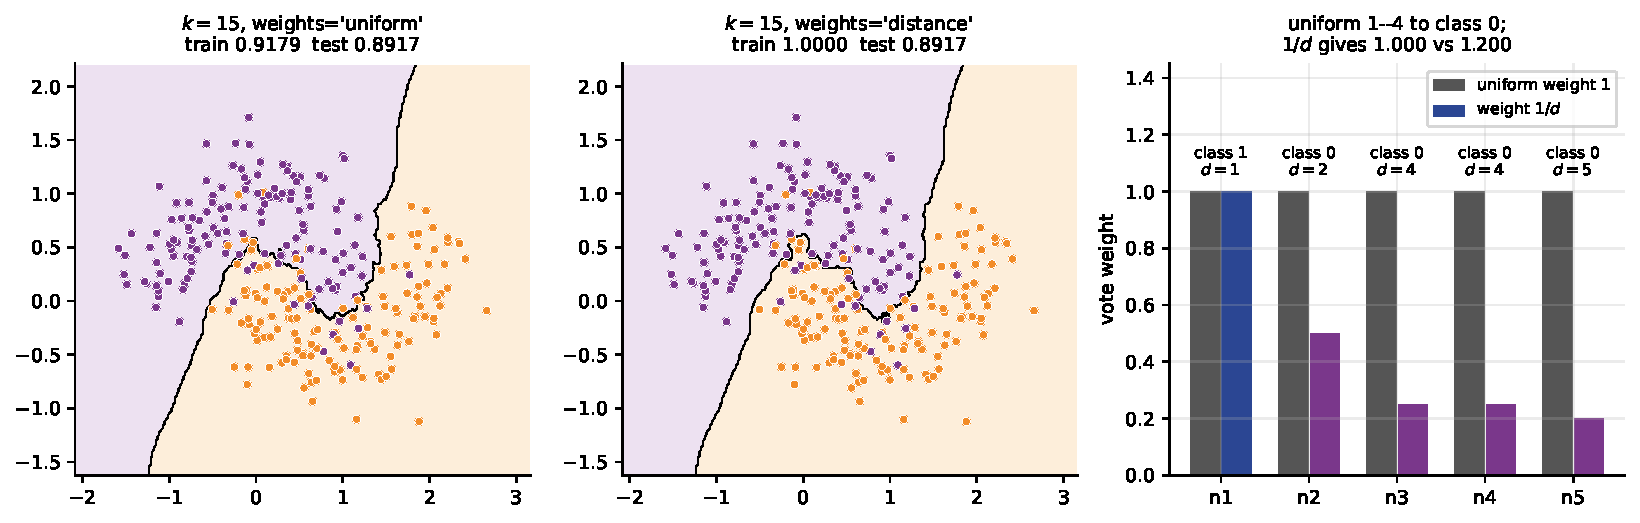
\includegraphics[width=\textwidth]{weighted-voting.pdf}
\caption{Left and centre: $k=15$ with uniform and with distance weights. The
weighted version reaches a training accuracy of $1.0000$ even at $k=15$,
because a training point is at distance $0$ from itself and $1/0$ is infinite.
Right: the five-neighbour hand calculation.}
\label{fig:weights}
\end{figure}

\begin{lstlisting}
for nm, d in [...]:
    for wt in ("uniform", "distance"):
        pipe = make_pipeline(StandardScaler(),
                             KNeighborsClassifier(15, weights=wt))
\end{lstlisting}
\begin{codeout}
dataset             uniform   distance     gain
iris                 0.9533     0.9533  +0.0000
wine                 0.9665     0.9608  -0.0057
breast_cancer        0.9613     0.9649  +0.0035
digits               0.9622     0.9627  +0.0006
training accuracy of k=25 with distance weights: 1.0000
\end{codeout}

Report that honestly: distance weighting is worth between $-0.0057$ and
$+0.0035$ here. It is not a free win. Its real value is elsewhere --- it never
produces a tie, it degrades gracefully when $k$ is too large, and it lets you
use a generous $k$ without washing out local structure.

\begin{caution}[Distance weighting makes every $k$ memorise]
Look at the last line: with \texttt{weights='distance'}, $k=25$ still scores
$1.0000$ on its own training set. A training point is at distance $0$ from
itself, its weight is infinite, and it outvotes everything. The training score
of a distance-weighted $k$-NN is $1.0$ for \emph{every} $k$, so it is even less
informative than usual.
\end{caution}

% =========================================================================
\section{The curse of dimensionality}
\label{sec:curse}

\subsection{Nearest and farthest become the same thing}

$k$-NN rests on one assumption: that ``near'' means something. In high
dimensions it stops meaning anything.

\begin{lstlisting}
rng = np.random.default_rng(0)
for d in (1, 2, 5, 10, 20, 50, 100, 500, 1000):
    for _ in range(20):
        Xr = rng.random((500, d)); qr = rng.random(d)
        dd = np.sqrt(((Xr - qr) ** 2).sum(axis=1))
        # record dd.min(), dd.max(), (dd.max() - dd.min()) / dd.min()
\end{lstlisting}
\begin{codeout}
   d   mean d_min   mean d_max   d_max/d_min   (max-min)/min
   1       0.0007       0.7705    1156.2859       3577.0046
   2       0.0177       0.9949      56.3273         85.5474
   5       0.1913       1.4461       7.5594          7.0526
  10       0.5743       1.9077       3.3218          2.3636
  20       1.0921       2.4688       2.2605          1.2790
  50       2.1574       3.4987       1.6217          0.6240
 100       3.3890       4.7604       1.4046          0.4053
 500       8.4577       9.7935       1.1579          0.1580
1000      12.2313      13.6006       1.1119          0.1120
\end{codeout}

Five hundred points drawn uniformly at random, and one query. In one dimension
the farthest point is over a thousand times as far away as the nearest. In a
thousand dimensions it is $1.11$ times as far. The nearest neighbour is barely
nearer than the farthest, and a classifier whose whole mechanism is ``find the
nearest'' has nothing left to work with.

\begin{figure}[htbp]
\centering

\includegraphics[width=\textwidth]{curse.pdf}
\caption{Left: the ratio $d_{\max}/d_{\min}$ collapses towards $1$ as the
dimension grows. Centre: both distances grow, and the gap between them stops
being a meaningful fraction of either. Right: the edge length a neighbourhood
must have to enclose a fixed fraction of the volume.}
\label{fig:curse}
\end{figure}

\subsection{Why: there is no such thing as ``local'' in high dimensions}

Here is the second way to see it, and it is the one to reproduce in an
examination.

\begin{worked}[How big is a small neighbourhood?]
Suppose the data fill the unit cube $[0,1]^d$ uniformly, and you want a
neighbourhood containing $1\%$ of the points. Take a small cube of edge $e$.
Its volume is $e^d$, so you need $e^d = 0.01$, that is $e = 0.01^{1/d}$.

\begin{center}\small
\begin{tabular}{@{}lrrrrrrr@{}}
\toprule
$d$ & 1 & 2 & 5 & 10 & 20 & 50 & 100\\
\midrule
$e = 0.01^{1/d}$ & $0.0100$ & $0.1000$ & $0.3981$ & $0.6310$ & $0.7943$ &
  $0.9120$ & $0.9550$\\
\bottomrule
\end{tabular}
\end{center}

In $100$ dimensions, capturing $1\%$ of your data requires a box spanning
$95.5\%$ of the range of \emph{every single feature}. It is not a
neighbourhood; it is nearly the whole dataset. \textbf{The word ``local'' has
no meaning in high dimensions}, and $k$-NN is a purely local method.
\end{worked}

\subsection{And it is not just about geometry: irrelevant features}

The abstract version is unsettling; this version is the one that will actually
happen to you. Take \texttt{iris}, whose four measurements do a fine job, and
bolt on columns of pure noise.

\begin{lstlisting}
rng2 = np.random.default_rng(0)          # the one seed for this lecture
for extra in (0, 2, 5, 10, 25, 50, 100, 200, 400):
    Xn = np.hstack([iris.data, rng2.normal(size=(150, extra))])
    knn  = cross_val_score(make_pipeline(StandardScaler(),
                                         KNeighborsClassifier(5)), Xn, yi, cv=CV).mean()
    tree = cross_val_score(DecisionTreeClassifier(random_state=0), Xn, yi, cv=CV).mean()
    lr   = cross_val_score(make_pipeline(StandardScaler(),
                                         LogisticRegression(max_iter=5000)), Xn, yi, cv=CV).mean()
\end{lstlisting}
\begin{codeout}
noise cols    KNN(5)     tree   logistic
        0    0.9533   0.9333     0.9600
        2    0.8800   0.9333     0.9400
        5    0.8333   0.9333     0.9667
       10    0.8267   0.9200     0.9400
       25    0.8133   0.9267     0.9333
       50    0.6867   0.9000     0.7600
      100    0.5333   0.9200     0.6800
      200    0.4667   0.9133     0.7000
      400    0.5200   0.9067     0.6067
\end{codeout}

\begin{figure}[htbp]
\centering
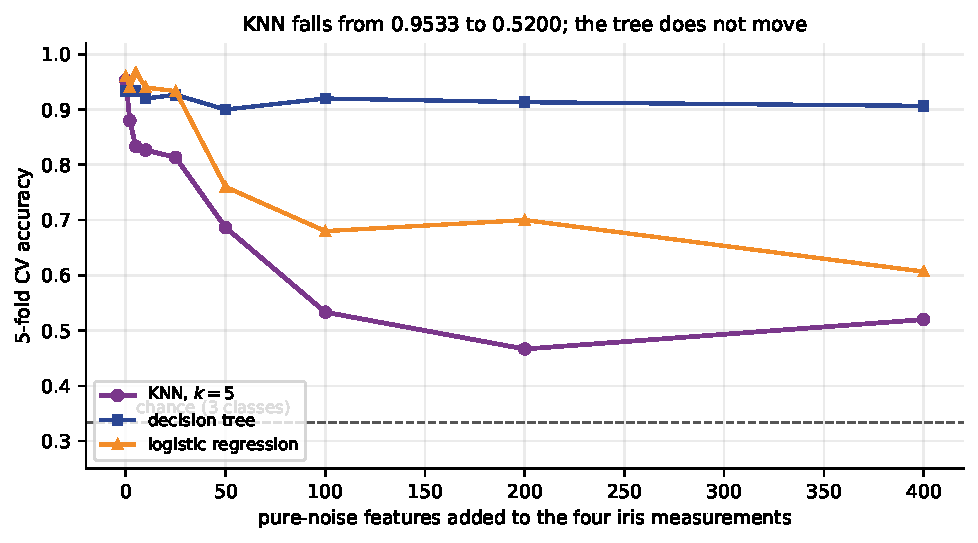
\includegraphics[width=0.72\textwidth]{noise-features.pdf}
\caption{Adding columns of pure noise to the four real iris measurements.
$k$-NN falls from $0.9533$ to $0.5200$; the decision tree barely moves.}
\label{fig:noise}
\end{figure}

$k$-NN falls from $0.9533$ to $0.5200$, bottoming out at $0.4667$ with $200$
noise columns --- about half its accuracy gone, and closing on the
one-in-three chance level. \emph{Two} noise columns already cost it seven
points. The last two rows move slightly the wrong way; read nothing into that,
the differences are one or two flowers out of $150$ and the fall is what
matters. The decision tree ends at $0.9067$, essentially where it started.

\begin{keyidea}
A decision tree \emph{chooses} which feature to split on and can ignore the
useless ones. $k$-NN cannot: every feature enters the distance sum with equal
weight, whether or not it carries any information. \textbf{$k$-NN has no
feature selection built in, so you must do it yourself.}
\end{keyidea}

That is the practical instruction. Before running $k$-NN on a wide table, use
the feature-selection tools from the preprocessing unit, or reduce with PCA,
or use a model that selects for you. Adding a column costs $k$-NN accuracy
unless that column earns its place.

% =========================================================================
\section{Ties, imbalance, and the rest of the failure list}
\label{sec:practical}

\subsection{Ties}

Two kinds of tie can occur. A \textbf{vote tie}, when $k$ is even and the
classes split evenly; and a \textbf{distance tie}, when the $k$th and
$(k{+}1)$th neighbours are equidistant so the neighbourhood itself is
ambiguous.

\begin{lstlisting}
Xt = np.array([[0.,0.], [2.,0.], [0.,2.], [2.,2.]])
yt = np.array([0, 1, 1, 0])
qt = np.array([[1., 1.]])                     # the exact centre
mt = KNeighborsClassifier(4).fit(Xt, yt)
print(mt.kneighbors(qt)[0], yt[mt.kneighbors(qt)[1][0]])
print(mt.predict_proba(qt)[0], mt.predict(qt)[0])
\end{lstlisting}
\begin{codeout}
all four neighbours at distance [1.4142 1.4142 1.4142 1.4142]
their labels [0 1 1 0]
k=4 probabilities [0.5 0.5] -> predict 0
k=2 probabilities [0.5 0.5] -> predict 0
k=3 probabilities [0.33333333 0.66666667] -> predict 1
\end{codeout}

\begin{keyidea}
scikit-learn breaks a tie \textbf{deterministically, in favour of the class
with the smaller label} --- it takes the \texttt{argmax} of the vote counts,
which returns the first maximum. It does not toss a coin and it does not warn
you.
\end{keyidea}

Three consequences worth knowing.

\begin{itemize}[leftmargin=*]
  \item \textbf{Use an odd $k$ for two classes.} It makes a vote tie
    impossible. Note the $k=2$ row above: it scored $0.9491$ in
    Section~\ref{sec:k}, below both $k=1$ and $k=3$ --- even $k$ is a small,
    avoidable handicap.
  \item \textbf{An odd $k$ does not help with three or more classes.} With
    $k=9$ and three classes a $3$:$3$:$3$ split is perfectly possible.
  \item \textbf{Distance ties are silently broken by row order.} Note that the
    $k=2$ case above chose two of four equidistant points, purely by index.
    Reordering the training rows can change the prediction.
\end{itemize}

The cleanest general fix is \texttt{weights='distance'}, which makes an exact
tie vanishingly unlikely.

\subsection{Imbalanced classes}

\begin{lstlisting}
X2, y2 = make_classification(n_samples=2000, n_features=10, n_informative=4,
                             n_redundant=0, weights=[0.95, 0.05],
                             flip_y=0.01, class_sep=1.0, random_state=0)
for k in (1, 3, 5, 15, 51, 151):
    m = KNeighborsClassifier(k).fit(A, ytr)
    pr = m.predict(B)
    print(k, accuracy_score(yte, pr), recall_score(yte, pr, pos_label=1),
          (pr == 1).sum())
\end{lstlisting}
\begin{codeout}
class counts [1882  118]
   k   accuracy   minority recall   minority predicted
   1     0.9367            0.4000               31
   3     0.9483            0.2571               14
   5     0.9550            0.2571               10
  15     0.9417            0.0000                0
  51     0.9417            0.0000                0
 151     0.9417            0.0000                0
always predicting the majority class scores 0.9417
k=51 with distance weights: accuracy 0.9417, minority recall 0.0000
\end{codeout}

\begin{figure}[htbp]
\centering
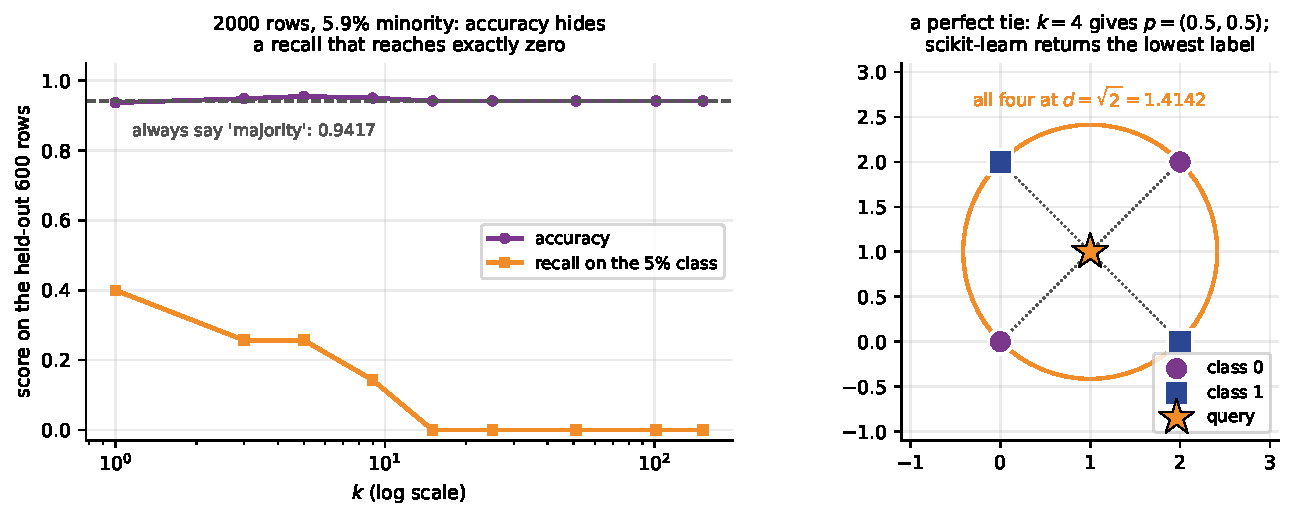
\includegraphics[width=\textwidth]{imbalance-and-ties.pdf}
\caption{Left: on a $94$:$6$ problem, accuracy stays around $0.94$ for every
$k$ while recall on the minority class falls to exactly zero. Right: the
four-way distance tie.}
\label{fig:imbalance}
\end{figure}

This is the most important table in the section. At $k=15$ and above the
classifier predicts the minority class \textbf{zero times} on $600$ held-out
rows, and its accuracy is $0.9417$ --- exactly the majority-class baseline. It
has learned nothing and it looks like it scores $94\%$.

The mechanism is arithmetic, not mystery. If the minority is $6\%$ of the data,
then in a neighbourhood of $51$ points drawn from anywhere the expected
minority count is about $3$. To win a vote it needs $26$. Only in a region of
overwhelming minority density can that happen, and with $118$ minority rows
spread over ten dimensions there is no such region.

\begin{caution}[Never report accuracy alone on imbalanced data]
$0.9417$ and $0.0000$ describe the same classifier. Report recall, precision
and the confusion matrix; and where a positive is what you care about, choose
the model on recall or on the F-score, not on accuracy.
\end{caution}

Three fixes, in order of preference: resample the training set (the
oversampling and undersampling methods from the preprocessing unit); use
\texttt{predict\_proba} with a threshold below $0.5$ rather than
\texttt{predict}; or choose an algorithm that supports
\texttt{class\_weight='balanced'} --- which \texttt{KNeighborsClassifier}, note,
does not.

\subsection{The complete failure list}

\begin{center}\small
\begin{tabular}{@{}p{4.0cm}p{4.2cm}p{5.2cm}@{}}
\toprule
\textbf{Failure} & \textbf{Symptom} & \textbf{Fix}\\
\midrule
unscaled features & one column supplies $90\%$ of the distance &
  \texttt{StandardScaler} in a \texttt{Pipeline}\\
$k$ too small & training $1.0$, test much lower & raise $k$; cross-validate\\
$k$ too large & accuracy equals the baseline & lower $k$\\
even $k$, two classes & silent tie-breaking & use an odd $k$, or
  \texttt{weights='distance'}\\
irrelevant features & accuracy falls as columns are added &
  feature selection, or PCA\\
high dimension & all distances nearly equal & reduce $d$; consider another
  algorithm\\
imbalanced classes & minority recall $0$, accuracy high & resample; move the
  threshold\\
slow prediction & latency grows with $n$ & index in low $d$; or use an eager
  learner\\
large model & the training data ships with the model & use an eager learner\\
missing values & \texttt{nan} propagates into every distance & impute before
  fitting\\
categorical features & ``distance'' between two words &
  encode first, or use a mixed metric\\
\bottomrule
\end{tabular}
\end{center}

\subsection{When $k$-NN is the right answer}

Given that list, why teach it? Four reasons, and they are real.

\begin{enumerate}[leftmargin=*]
  \item \textbf{It is the honest baseline.} It has one hyperparameter and no
    assumptions. If your elaborate model cannot beat $k$-NN, the elaborate
    model is not earning its keep.
  \item \textbf{It makes no assumption about the shape of the boundary.} Given
    enough data, 1-NN's error rate is provably no worse than twice the best
    possible error rate of any classifier --- the classical Cover--Hart result.
    Few algorithms come with a guarantee that clean.
  \item \textbf{It is naturally multi-class.} Ten classes need no extra
    machinery; contrast logistic regression, which needs one-vs-rest or
    softmax. On \texttt{digits}, $k$-NN scored $0.9796$ against logistic
    regression's $0.9611$.
  \item \textbf{It extends to problems with no feature vector at all}, as long
    as you can define a distance --- edit distance between strings, dynamic time
    warping between signals, graph distance. This is why it survives in
    recommender systems and in retrieval.
\end{enumerate}

% =========================================================================
\section{Summary}
\label{sec:summary}

\begin{enumerate}[leftmargin=*]
  \item Classification predicts a label from a finite set. Han, Kamber and
    Pei's general approach has two steps: model construction from a labelled
    training set, then model usage, with accuracy estimated on an independent
    test set.
  \item An \textbf{eager} learner works at fit time; a \textbf{lazy} or
    \textbf{instance-based} learner works at predict time. Measured on
    \texttt{digits}, in operation counts rather than seconds: per prediction
    $k$-NN does $125.7$ times the arithmetic logistic regression does, and its
    \texttt{fit} does none at all.
  \item $k$-NN stores the training set. On \texttt{digits} that is $643{,}584$
    bytes against $5{,}200$ for logistic regression's coefficients ---
    $124\times$ more, and growing with $n$.
  \item Multiplying the training set by $40$ multiplies $k$-NN's distance
    computations by exactly $40$, and leaves logistic regression's prediction
    cost unchanged.
  \item The algorithm is: distance to every training point, keep the $k$
    smallest, vote. Worked by hand on seven points, $1$-NN put $q_1 = (3,3)$ in
    class $0$ via neighbour $B$ at $d = \sqrt{2}$ --- and
    \texttt{KNeighborsClassifier} returned $1.414214$ and class $0$.
  \item $k$ changes the answer. On $q_2 = (6,3)$: $k=1 \to 0$, $k=3 \to 1$,
    $k=5 \to 1$, $k=7 \to 0$. At $k = n$ the classifier is the majority-class
    baseline.
  \item \textbf{$k=1$ scores exactly $1.000000$ on its own training set},
    because every training row is its own nearest neighbour at distance $0$.
    Training accuracy is worthless as evidence here.
  \item The validation curve is U-shaped: on \texttt{breast\_cancer} it peaks
    at $k=11$ with $0.9666$ and falls to $0.6274$ --- the baseline --- at
    $k=398$. The peak is shallow: $k=3$ to $k=15$ are indistinguishable.
  \item Small $k$ is low bias and high variance; large $k$ is the reverse. The
    effective number of parameters is about $n/k$.
  \item \textbf{Scaling.} On two \texttt{breast\_cancer} patients, \emph{mean
    area} alone supplied $90.4482\%$ of the squared distance and the twenty-seven
    non-area columns shared $0.7655\%$. Standardising changed the nearest
    neighbour of $164$ of $171$ test patients and the predicted class of $19$.
  \item Measured gains from \texttt{StandardScaler} at $k=5$: \texttt{wine}
    $+0.2975$, \texttt{breast\_cancer} $+0.0334$, \texttt{iris} $+0.0000$,
    \texttt{digits} $\mathbf{-0.0089}$. Scale when the units differ; not
    reflexively.
  \item Minkowski-$p$ contains Manhattan ($p{=}1$), Euclidean ($p{=}2$) and
    Chebyshev ($p{\to}\infty$). For $q=(0,0)$, $P=(3,0)$, $Q=(2,2)$ the nearest
    neighbour is $P$ under $L_1$ and $Q$ under $L_2$; the crossover is at
    $p^\ast = 1/(\log_2 3 - 1) = 1.7095$. On real standardised data the choice
    moves accuracy by under $0.01$.
  \item Distance weighting ($1/d$) turned a $4$:$1$ uniform vote into a
    $1.2$:$1.0$ weighted one. Measured, it is worth between $-0.0057$ and
    $+0.0035$ --- and it makes \emph{every} $k$ score $1.0$ on the training set.
  \item \textbf{The curse of dimensionality.} With $500$ uniform points, the
    farthest is $1156\times$ the nearest at $d=1$ and $1.11\times$ at
    $d=1000$. A box holding $1\%$ of the data in $100$ dimensions must span
    $95.5\%$ of every feature's range.
  \item Adding pure-noise columns to \texttt{iris} took $k$-NN from $0.9533$
    to $0.5200$, with a low of $0.4667$; a decision tree went from $0.9333$ to
    $0.9067$. $k$-NN has no built-in feature selection.
  \item Ties are broken deterministically towards the lowest class label. Use
    an odd $k$ for two classes; it does not help for three.
  \item On a $94$:$6$ problem, $k \ge 15$ predicted the minority class zero
    times in $600$ rows while scoring $0.9417$ --- exactly the baseline. Never
    report accuracy alone.
  \item $k$-NN remains the right first thing to try: one hyperparameter, no
    assumptions about the boundary, naturally multi-class, and usable wherever
    a distance can be defined.
\end{enumerate}

% =========================================================================
\section{Practice questions}
\label{sec:practice}

Attempt them before reading Section~\ref{sec:solutions}. Questions 1, 2 and 5
are of the type the class test asks; do those with a pen, not a laptop.

\begin{enumerate}[leftmargin=*, itemsep=0.55em]

\item \textbf{(1-NN, 3-NN and 5-NN by hand.)} A training set of six instances
  with two features and two classes:

  \begin{center}\small
  \begin{tabular}{@{}lrrl@{}}
  \toprule
  point & $x_1$ & $x_2$ & class\\
  \midrule
  $P_1$ & 1 & 2 & A\\
  $P_2$ & 2 & 5 & A\\
  $P_3$ & 3 & 1 & A\\
  $P_4$ & 5 & 4 & B\\
  $P_5$ & 6 & 6 & B\\
  $P_6$ & 8 & 3 & B\\
  \bottomrule
  \end{tabular}
  \end{center}

  Classify $q = (4, 4)$ using Euclidean distance. Give the full table of
  squared distances, the ranking, and the predictions for $k=1$, $k=3$ and
  $k=5$. Explain in one sentence why the answer changes.

\item \textbf{(Distance-weighted voting by hand.)} Using the same six points
  and the same query, apply distance weighting with weight $1/d$ at $k=5$.
  Give both class totals to four decimal places and the prediction. Does
  weighting agree with the uniform $5$-NN answer of question 1?

\item \textbf{(Eager and lazy.)} Classify each of the following as an eager or
  a lazy learner, and give the one-line reason:
  logistic regression; $k$-nearest neighbour; a decision tree; na\"ive Bayes; a
  support vector machine; a distance-weighted $k$-NN with $k=1$.
  Then: a hospital wants a classifier that answers within $10$\,ms on a
  training set of $2$ million patient records, and cannot let the records
  leave the building. Which family should it use, and why? Cite two measured
  numbers from these notes.

\item \textbf{(Why scaling.)} Two customers are recorded as
  $p = (\text{age }25,\ \text{income }30000)$ and
  $q = (\text{age }45,\ \text{income }32000)$, income in rupees.
  \begin{enumerate}[label=(\alph*)]
    \item Compute the squared Euclidean distance and the percentage of it
      contributed by each feature.
    \item Now standardise using training statistics: age has mean $35$ and
      standard deviation $10$; income has mean $31000$ and standard deviation
      $1000$. Recompute the squared distance and the percentage contributed by
      each feature.
    \item State in one sentence what standardising did to the question ``who
      is my nearest neighbour?''
  \end{enumerate}

\item \textbf{(Minkowski crossover.)} Query $q = (0,0)$; candidates
  $P = (5, 0)$ of class $0$ and $Q = (3, 3)$ of class $1$.
  \begin{enumerate}[label=(\alph*)]
    \item Give the $1$-NN prediction under Manhattan distance and under
      Euclidean distance.
    \item Find the exact value of $p$ at which the two candidates are
      equidistant under the Minkowski metric. Give it to four decimal places.
    \item What does Chebyshev distance ($p \to \infty$) say?
  \end{enumerate}

\item \textbf{(The curse, quantitatively.)} Data fill the unit cube
  $[0,1]^d$ uniformly.
  \begin{enumerate}[label=(\alph*)]
    \item What edge length must a cubical neighbourhood have to contain
      $10\%$ of the data when $d = 20$?
    \item And to contain $50\%$ when $d = 10$?
    \item Explain in two sentences why this makes $k$-NN unreliable in high
      dimensions, using the phrase ``no longer local''.
  \end{enumerate}

\item \textbf{(Reading a validation curve.)} A student reports the following
  cross-validated accuracies for a two-class problem with $n = 400$ training
  rows: $k=1$: $0.831$; $k=5$: $0.878$; $k=15$: $0.884$; $k=45$: $0.869$;
  $k=200$: $0.771$; $k=400$: $0.640$.
  \begin{enumerate}[label=(\alph*)]
    \item Which end of the curve is high variance and which is high bias?
    \item What, almost certainly, is the class balance of the dataset? How do
      you know?
    \item The student also reports a training accuracy of $1.000$ at $k=1$ and
      concludes that $k=1$ ``fits the data perfectly''. Correct them.
  \end{enumerate}

\item \textbf{(Ties.)} A binary problem, $k = 6$, and the six nearest
  neighbours of a query split $3$:$3$.
  \begin{enumerate}[label=(\alph*)]
    \item What does \texttt{KNeighborsClassifier} predict, and by what rule?
    \item Give two different changes to the model that would remove the
      ambiguity, and say what each costs.
    \item Would using an odd $k$ guarantee no ties on a five-class problem?
  \end{enumerate}

\item \textbf{(Debugging.)} A classmate writes:

\begin{lstlisting}
X = StandardScaler().fit_transform(bc.data)
Xtr, Xte, ytr, yte = train_test_split(X, bc.target, random_state=0)
knn = KNeighborsClassifier(n_neighbors=1).fit(Xtr, ytr)
print("accuracy", knn.score(Xtr, ytr))       # prints 1.0
\end{lstlisting}

  and reports ``$k$-NN achieves 100\% accuracy on breast cancer data''. % chktex 36
  Identify three separate problems with this and give the corrected code.

\item \textbf{(Irrelevant features.)} A colleague has a table of $80$ patients
  and $3000$ gene-expression measurements, of which perhaps a dozen are
  relevant. They plan to use $k$-NN with $k=5$ and Euclidean distance.
  Predict what will happen, quoting the relevant measurement from these notes,
  and propose two concrete changes to the plan.

\end{enumerate}

% =========================================================================
\section{Solutions}
\label{sec:solutions}

\begin{enumerate}[leftmargin=*, itemsep=0.7em]

\item Squared distances from $q = (4,4)$:

  \begin{center}\small
  \begin{tabular}{@{}lrrrrrr@{}}
  \toprule
  point & $P_1$ & $P_2$ & $P_3$ & $P_4$ & $P_5$ & $P_6$\\
  \midrule
  $(x_1-4)^2$ & 9 & 4 & 1 & 1 & 4 & 16\\
  $(x_2-4)^2$ & 4 & 1 & 9 & 0 & 4 & 1\\
  \midrule
  $d^2$ & 13 & 5 & 10 & \textbf{1} & 8 & 17\\
  $d$ & 3.6056 & 2.2361 & 3.1623 & \textbf{1.0000} & 2.8284 & 4.1231\\
  class & A & A & A & B & B & B\\
  \bottomrule
  \end{tabular}
  \end{center}

  Ranking: $P_4$ (B), $P_2$ (A), $P_5$ (B), $P_3$ (A), $P_1$ (A), $P_6$ (B).

  \begin{itemize}
    \item $k=1$: $\{P_4\}$ $\to$ \textbf{B}.
    \item $k=3$: $\{P_4, P_2, P_5\}$ = B, A, B $\to$ $2$:$1$ $\to$ \textbf{B}.
    \item $k=5$: $\{P_4, P_2, P_5, P_3, P_1\}$ = B, A, B, A, A $\to$ A gets
      $3$, B gets $2$ $\to$ \textbf{A}.
  \end{itemize}

  The answer changes because the query sits near the boundary. Widening the
  neighbourhood reaches back into the dense class-A region on the left, and
  three moderately distant A points outvote two near B points --- a uniform
  vote does not care how far away a neighbour is.

\item Weights $1/d$ for the five nearest, from the table above:

  \begin{center}\small
  \begin{tabular}{@{}lrrrrr@{}}
  \toprule
  neighbour & $P_4$ & $P_2$ & $P_5$ & $P_3$ & $P_1$\\
  \midrule
  class & B & A & B & A & A\\
  $d$ & 1.0000 & 2.2361 & 2.8284 & 3.1623 & 3.6056\\
  $1/d$ & 1.0000 & 0.4472 & 0.3536 & 0.3162 & 0.2774\\
  \bottomrule
  \end{tabular}
  \end{center}

  Class A: $0.4472 + 0.3162 + 0.2774 = \mathbf{1.0408}$.
  Class B: $1.0000 + 0.3536 = \mathbf{1.3536}$.
  Prediction: \textbf{B}.

  No, it disagrees with the uniform $5$-NN answer of A. The single very close
  B neighbour at $d = 1$ carries more weight on its own than any two of the A
  neighbours together. Verified in code:
  \texttt{KNeighborsClassifier(5, weights='distance')} returns class B.

\item \emph{Eager}: logistic regression (fits a weight vector, then discards
  the data); decision tree (builds a tree structure); na\"ive Bayes (estimates
  class-conditional means and variances); SVM (solves a quadratic programme for
  the support vectors and their coefficients). \emph{Lazy}: $k$-NN, and
  distance-weighted $1$-NN --- weighting changes the vote, not the timing of the
  work.

  The hospital should use an \textbf{eager} learner. Two measured reasons.
  \textbf{Latency}: $k$-NN's prediction cost grows linearly with $n$, and
  this is arithmetic rather than benchmarking --- $40\times$ the training rows
  is exactly $40\times$ the distance computations, $10{,}000{,}000$ against
  $250{,}000$ at $20{,}000$ rows. Two million rows means a hundred times that
  again for every single answer, which no $10$\,ms budget survives; logistic
  regression's prediction does not touch the training rows at all, so its
  cost does not move.
  \textbf{Data residency}: a fitted $k$-NN \emph{is} the training data ---
  $643{,}584$ bytes of patient records on \texttt{digits} against $5{,}200$
  bytes of coefficients --- so deploying it means deploying the records.

\item
  \begin{enumerate}[label=(\alph*)]
    \item $\Delta\text{age} = 20$, so $400$. $\Delta\text{income} = 2000$, so
      $4{,}000{,}000$. Total $= 4{,}000{,}400$. Income contributes
      $4000000/4000400 = \mathbf{99.99\%}$; age contributes
      $\mathbf{0.01\%}$.
    \item Standardised: $p_z = ((25-35)/10,\ (30000-31000)/1000) = (-1, -1)$
      and $q_z = ((45-35)/10,\ (32000-31000)/1000) = (+1, +1)$. Differences
      are $-2$ and $-2$; squared, $4$ and $4$; total $\mathbf{8}$. Each
      feature now contributes \textbf{exactly $50\%$}.
    \item Before standardising, ``nearest neighbour'' meant ``the customer with
      the most similar income''; age was not consulted. After standardising it
      means ``the customer most similar in both'', because a one-standard-deviation
      move counts the same in either column.
  \end{enumerate}

\item
  \begin{enumerate}[label=(\alph*)]
    \item Manhattan: $d_1(q,P) = 5 + 0 = 5$; $d_1(q,Q) = 3 + 3 = 6$. Nearest
      is $P$ $\to$ \textbf{class 0}. Euclidean: $d_2(q,P) = 5$;
      $d_2(q,Q) = \sqrt{9+9} = \sqrt{18} = 4.2426$. Nearest is $Q$ $\to$
      \textbf{class 1}.
    \item Set $5 = (3^p + 3^p)^{1/p} = 3 \cdot 2^{1/p}$. Then
      $2^{1/p} = 5/3$, so $1/p = \log_2(5/3)$ and
      \[
        p^\ast = \frac{1}{\log_2(5/3)} = \mathbf{1.3569}.
      \]
      Below $1.3569$ the prediction is class $0$; above it, class $1$.
      (Check: at $p = 1.3569$ both distances are $5.0000$.)
    \item Chebyshev takes the largest coordinate difference: $\max(5,0) = 5$
      for $P$ and $\max(3,3) = 3$ for $Q$. Nearest is $Q$ $\to$ class $1$,
      consistent with every $p > 1.3569$.
  \end{enumerate}

\item
  \begin{enumerate}[label=(\alph*)]
    \item $e = 0.10^{1/20} = \mathbf{0.8913}$ --- the box must span $89\%$ of
      every one of the twenty features.
    \item $e = 0.50^{1/10} = \mathbf{0.9330}$.
    \item To contain enough neighbours to average over, a neighbourhood in high
      dimensions must be so wide that it is \textbf{no longer local}: it spans
      almost the entire range of every feature. $k$-NN's whole premise is that
      nearby points share a label, and when ``nearby'' covers the whole dataset
      that premise is empty --- which is the same fact the $d_{\max}/d_{\min}
      \to 1$ measurement reports from the other direction.
  \end{enumerate}

\item
  \begin{enumerate}[label=(\alph*)]
    \item Small $k$ is \textbf{high variance}, low bias: $k=1$ at $0.831$ is
      fitting noise. Large $k$ is \textbf{high bias}, low variance: $k=200$ and
      $k=400$ are over-smoothing.
    \item At $k = 400 = n$ the classifier is exactly the majority-class
      baseline, so its accuracy \emph{is} the majority-class proportion:
      about \textbf{$64\%$ / $36\%$}. This is a free diagnostic --- read the
      right-hand end of any $k$-NN validation curve and you have the class
      balance.
    \item A training accuracy of $1.000$ at $k=1$ is guaranteed by arithmetic:
      every training row is its own nearest neighbour, at distance $0$, so it
      recites its own label. It happens on every dataset, including one with
      random labels, and is not evidence of anything. The relevant number is
      the cross-validated $0.831$ --- which is the \emph{worst} entry in the
      whole table.
  \end{enumerate}

\item
  \begin{enumerate}[label=(\alph*)]
    \item It predicts the class with the \textbf{lower label} (class $0$ in a
      $\{0,1\}$ problem). \texttt{predict\_proba} returns
      \texttt{[0.5, 0.5]} and \texttt{predict} takes the \texttt{argmax}, which
      returns the \emph{first} maximum. It is deterministic and silent.
    \item (i) Use an odd $k$ ($5$ or $7$): costs nothing, and removes vote ties
      entirely for two classes. (ii) Use \texttt{weights='distance'}: an exact
      tie then requires the two groups' reciprocal distances to sum to exactly
      the same value, which is vanishingly unlikely --- but it makes the training
      score $1.0$ for every $k$ and gives the nearest neighbour a great deal of
      influence.
    \item No. With five classes and $k = 15$, a $3$:$3$:$3$:$3$:$3$ split is a
      tie, and odd $k$ does nothing about it. Odd $k$ only guarantees no tie
      when there are exactly two classes.
  \end{enumerate}

\item Three problems.

  \begin{enumerate}[label=(\roman*)]
    \item \textbf{The score is on the training set.} \texttt{knn.score(Xtr,
      ytr)} at $k=1$ is $1.0$ by construction. It measures nothing.
    \item \textbf{The scaler was fitted on all the data before splitting.}
      \texttt{StandardScaler().fit\_transform(bc.data)} learns the mean and
      standard deviation of the test rows too. On this dataset the leak is
      small, but the habit is the one that produces large leaks elsewhere; the
      correct place for a scaler is inside a \texttt{Pipeline}.
    \item \textbf{$k=1$ was not chosen, it was assumed.} $k$ is the only
      hyperparameter this model has, and cross-validation on
      \texttt{breast\_cancer} prefers $k=11$ ($0.9666$ against $0.9578$).
  \end{enumerate}

  Corrected:

\begin{lstlisting}
from sklearn.model_selection import GridSearchCV, StratifiedKFold
pipe = make_pipeline(StandardScaler(), KNeighborsClassifier())
grid = GridSearchCV(pipe, {"kneighborsclassifier__n_neighbors":
                           [1, 3, 5, 7, 11, 15, 21, 31]},
                    cv=StratifiedKFold(5, shuffle=True, random_state=0))
Xtr, Xte, ytr, yte = train_test_split(bc.data, bc.target, test_size=0.3,
                                      random_state=0, stratify=bc.target)
grid.fit(Xtr, ytr)
print(grid.best_params_, grid.best_score_)
print("held-out accuracy", grid.score(Xte, yte))
\end{lstlisting}

  Note that the split now happens \emph{first}, the scaler is refitted inside
  every fold, $k$ is chosen on the training data only, and the reported number
  comes from rows the whole procedure has never seen.

\item It will fail, and it will fail badly. With $80$ rows and $3000$ columns,
  almost every column is noise, and $k$-NN weights every column equally in the
  distance. The measured analogue in these notes: adding $400$ pure-noise
  columns to the four real \texttt{iris} measurements took $k$-NN from
  $0.9533$ to $\mathbf{0.5200}$, having passed through $0.4667$ on the way,
  while a decision tree on the same tables went only from $0.9333$ to
  $0.9067$. Separately, $d_{\max}/d_{\min}$ for $500$ uniform points is
  $1.16$ at $d = 500$: in that regime the nearest neighbour is barely nearer
  than the farthest.

  Two concrete changes. \textbf{(i)} Put a feature-selection or
  dimensionality-reduction step in front of the classifier --- a univariate
  filter, or PCA to a few dozen components --- and fit it \emph{inside} the
  cross-validation folds, since with $80$ rows and $3000$ candidate columns
  selecting on all the data before splitting will manufacture accuracy out of
  nothing. \textbf{(ii)} Use an algorithm that selects features as part of
  fitting: an L1-regularised logistic regression, or a tree-based model. Then
  compare it against $k$-NN on the reduced feature set and report both.

\end{enumerate}

% =========================================================================
\section{References and further reading}
\label{sec:refs}

All links were checked on 23 August 2026. Free resources are marked
\textbf{[free]}.

\subsection*{Textbooks}

\begin{itemize}[leftmargin=*]
  \item Han, Kamber and Pei, \emph{Data Mining: Concepts and Techniques}, 3rd
    edition, Morgan Kaufmann, 2012. \textbf{A prescribed text, and the
    reference for the first half of this lecture.} \S8.1 ``Basic Concepts'' ---
    what classification is, the two-step general approach of
    Section~\ref{sec:twostep}, and classification against numeric prediction.
    \S9.5.1 ``$k$-Nearest-Neighbor Classifiers'' is the $k$-NN treatment in the
    vocabulary the examination uses, including lazy learners, the choice of
    $k$, distance-weighted voting and the handling of nominal attributes and
    missing values. \S8.5 has the confusion matrix, precision and recall used
    in Section~\ref{sec:setting}.
  \item M\"uller and Guido, \emph{Introduction to Machine Learning with
    Python}, O'Reilly, 2016. \textbf{The prescribed practical text.} Ch.~2
    ``Supervised Learning'' --- \S2.1 classification and regression, \S2.2
    generalisation, overfitting and underfitting (the model-complexity curve of
    Section~\ref{sec:k}), and \S2.3.1 ``$k$-Nearest Neighbors'', which is this
    lecture with the same \texttt{scikit-learn} API and the same $n\_neighbors$
    boundary plots. \S2.3.2 contrasts it with linear models. Notebooks
    \textbf{[free]}:
    \url{https://github.com/amueller/introduction_to_ml_with_python}
  \item James, Witten, Hastie, Tibshirani and Taylor, \emph{An Introduction to
    Statistical Learning with Python}. \textbf{[free]} \S2.2.3 ``The
    Classification Setting'' introduces $k$-NN and the Bayes error rate, with
    the figure showing $k=1$ against $k=100$ that Figure~\ref{fig:kbound}
    reproduces on different data; \S4.7.6 ``$K$-Nearest Neighbors'' places it
    beside logistic regression, LDA and QDA and says exactly when each wins;
    \S4.1 and \S4.2 are the ``why not linear regression'' argument for
    classification. \url{https://www.statlearning.com/}
  \item Bishop, \emph{Pattern Recognition and Machine Learning}, Springer,
    2006. \textbf{A prescribed text.} \S2.5.2 ``Nearest-neighbour methods'' ---
    $k$-NN derived from kernel density estimation, which explains why it is a
    non-parametric method rather than a heuristic; \S1.4 ``The Curse of
    Dimensionality'' is the volume argument of Section~\ref{sec:curse} done
    properly; \S1.5 is the decision-theory framing of a decision boundary.
  \item Murphy, \emph{Probabilistic Machine Learning: An Introduction}, MIT
    Press, 2022. \textbf{[free]} \S16.1 ``Exemplar-based models'' and
    \S16.1.1 on $k$-NN, including the Cover--Hart result quoted in
    Section~\ref{sec:practical} and \S16.1.2 on the curse of dimensionality
    with the same unit-cube calculation. \S16.2 covers learning the distance
    metric, which is where this lecture stops.
    \url{https://probml.github.io/pml-book/book1.html}
  \item Mitchell, \emph{Machine Learning}, McGraw Hill, 1997. Ch.~8
    ``Instance-Based Learning'' is the classical account, and the one most
    Indian syllabuses are written from: \S8.1 introduces the lazy/eager
    distinction, \S8.2 is $k$-NN including distance weighting and the
    inductive bias, and \S8.5 makes the ``lazy versus eager'' comparison in
    general terms.
  \item Hastie, Tibshirani and Friedman, \emph{The Elements of Statistical
    Learning}, 2e, Springer. \textbf{[free]} \S2.3.2 ``Nearest-Neighbor
    Methods'' and \S2.3.3, which compare $k$-NN with least squares on the same
    picture; \S13.3 is a full chapter section on prototype and
    nearest-neighbour methods, including the invariant metrics and editing
    rules for reducing the stored set.
    \url{https://hastie.su.domains/ElemStatLearn/}
\end{itemize}

\subsection*{Online courses}

\begin{sloppypar}
\begin{itemize}[leftmargin=*]
  \item \textbf{NPTEL, Introduction to Machine Learning} --- Prof.\ Balaraman
    Ravindran, IIT Madras. The reference course for the semester; the
    classification weeks cover the general setting, $k$-NN and the
    bias--variance reading of $k$. \textbf{[free]}
    \url{https://nptel.ac.in/courses/106106139}
  \item \textbf{NPTEL, Introduction to Machine Learning --- IITKGP} ---
    Prof.\ Sudeshna Sarkar, IIT Kharagpur. A second, shorter treatment of the
    same material; useful if Ravindran's pace does not suit you.
    \textbf{[free]} \url{https://nptel.ac.in/courses/106105152}
  \item \textbf{NPTEL, Data Mining} --- Prof.\ Pabitra Mitra, IIT Kharagpur.
    Follows Han, Kamber and Pei closely, so this is the closest match to the
    \emph{vocabulary} of Sections~\ref{sec:setting} and~\ref{sec:lazy} ---
    tuples, attributes, eager and lazy learners. \textbf{[free]}
    \url{https://nptel.ac.in/courses/106105174}
  \item \textbf{SWAYAM} --- the national portal hosting NPTEL. \textbf{[free]}
    \url{https://swayam.gov.in/}
  \item \textbf{Google Machine Learning Crash Course, Classification} ---
    seventy minutes on thresholds, the confusion matrix, accuracy, precision,
    recall, ROC and AUC. The right companion to Section~\ref{sec:setting} and
    the direct preparation for this unit's evaluation lecture. \textbf{[free]}
    \url{https://developers.google.com/machine-learning/crash-course/classification}
  \item \textbf{Kaggle Learn, Intro to Machine Learning} --- short browser
    lessons; the right warm-up if the \texttt{scikit-learn} fit/predict/score
    API is still unfamiliar. \textbf{[free]}
    \url{https://www.kaggle.com/learn/intro-to-machine-learning}
\end{itemize}
\end{sloppypar}

\subsection*{Videos}

\begin{itemize}[leftmargin=*]
  \item StatQuest with Josh Starmer, \emph{StatQuest: K-nearest neighbors,
    Clearly Explained} --- five minutes, and the clearest short account of the
    algorithm. Watch this one first if Section~\ref{sec:knn} did not land.
    \textbf{[free]} \url{https://youtu.be/HVXime0nQeI}
  \item Mahesh Huddar, \emph{1. Solved Numerical Example of KNN Classifier to
    classify New Instance IRIS Example} --- the distance table built on a
    whiteboard, in exactly the format the class test wants. Do
    Section~\ref{sec:hand} first and then watch this to check your method.
    \textbf{[free]} \url{https://youtu.be/Vk9lGGODaJA}
  \item Mahesh Huddar, \emph{Solved Example K Nearest Neighbors Algorithm
    Weighted KNN to classify New Instance} --- the distance-weighted vote of
    Section~\ref{sec:metric} worked out numerically. \textbf{[free]}
    \url{https://youtu.be/kCNpLbCUo7g}
  \item Mahesh Huddar, \emph{Part 2 --- K Nearest Neighbor KNN Solved Example
    Cosine Similarity Manhattan Distance} --- the same query under several
    metrics, which is Section~\ref{sec:crossover} with different numbers.
    \textbf{[free]} \url{https://youtu.be/w2FIg2-ln8s}
  \item Mahesh Huddar, \emph{3. K nearest Neighbor Learning Algorithm Lazy
    Learner Solved Example} --- the lazy-learner framing of
    Section~\ref{sec:eagerlazy}, in examination vocabulary. \textbf{[free]}
    \url{https://youtu.be/T0YkfWssHjk}
  \item StatQuest with Josh Starmer, \emph{Machine Learning Fundamentals: Bias
    and Variance} --- the trade-off that choosing $k$ is an instance of.
    \textbf{[free]} \url{https://youtu.be/EuBBz3bI-aA}
  \item StatQuest with Josh Starmer, \emph{Machine Learning Fundamentals: Cross
    Validation} --- how the curve in Figure~\ref{fig:kcurve} was produced, and
    why it is the number to trust. \textbf{[free]}
    \url{https://youtu.be/fSytzGwwBVw}
\end{itemize}

\subsection*{Documentation and interactive explainers}

\begin{itemize}[leftmargin=*]
  \item scikit-learn user guide, \emph{Nearest Neighbors} (\S1.6) --- the
    unsupervised and supervised neighbour machinery, the brute-force / KD-tree
    / ball-tree discussion behind Section~\ref{sec:lazy}, and
    \S1.6.5 on nearest-centroid classification. \textbf{[free]}
    \url{https://scikit-learn.org/stable/modules/neighbors.html}
  \item scikit-learn API reference, \texttt{KNeighborsClassifier} --- every
    parameter used in these notes: \texttt{n\_neighbors}, \texttt{weights},
    \texttt{p}, \texttt{metric}, \texttt{algorithm}. \textbf{[free]}
    \url{https://scikit-learn.org/stable/modules/generated/sklearn.neighbors.KNeighborsClassifier.html}
  \item scikit-learn example, \emph{Nearest Neighbors Classification} --- the
    uniform-against-distance boundary comparison of
    Figure~\ref{fig:weights}, on iris. \textbf{[free]}
    \url{https://scikit-learn.org/stable/auto_examples/neighbors/plot_classification.html}
  \item scikit-learn example, \emph{Classifier comparison} --- ten classifiers
    on three synthetic datasets; the published version of
    Figure~\ref{fig:landscape}, and the single most useful picture in the whole
    of Unit VI. \textbf{[free]}
    \url{https://scikit-learn.org/stable/auto_examples/classification/plot_classifier_comparison.html}
  \item scikit-learn example, \emph{Importance of Feature Scaling} --- the
    experiment of Section~\ref{sec:scale} run on the wine dataset, with a
    $k$-NN classifier. \textbf{[free]}
    \url{https://scikit-learn.org/stable/auto_examples/preprocessing/plot_scaling_importance.html}
  \item scikit-learn, \emph{Common pitfalls and recommended practices} --- read
    the inconsistent-preprocessing and data-leakage sections before you next
    report a score. \textbf{[free]}
    \url{https://scikit-learn.org/stable/common_pitfalls.html}
  \item MLU-Explain, \emph{The Bias Variance Tradeoff} --- an interactive
    explainer with a live $k$-NN example: drag $k$ and watch the boundary and
    both error curves move. This is Figure~\ref{fig:kcurve} that you can
    play with. \textbf{[free]}
    \url{https://mlu-explain.github.io/bias-variance/}
  \item MLU-Explain, \emph{Train, Test, and Validation Sets} and
    \emph{Precision \& Recall} --- the two-step workflow of
    Section~\ref{sec:twostep} and the confusion-matrix reading of
    Section~\ref{sec:setting}, both interactive. \textbf{[free]}
    \url{https://mlu-explain.github.io/train-test-validation/} \\
    \url{https://mlu-explain.github.io/precision-recall/}
\end{itemize}

\enlargethispage{4\baselineskip}
\notesources{\AMLUnitVISources}

\end{document}
